%% ergebnisse.tex

\chapter{Ergebnisse und Diskussion}
\label{ch:Ergebnisse}

\section{Allgemeine Merkmale des Netzwerkes}
\label{sec:result-allg-merkm-des}

\section{Eigenschaften einzelner Schl\"ussel}
\label{sec:result-key-properties}

\section{Zusammenhangskomponenten und Communities}
\label{sec:result-zusamm-und-comm}

\section{Struktur der starken Zusammenhangskomponenten}
\label{sec:result-komponentenstruktur}

\begin{figure}[t]
  \centering
  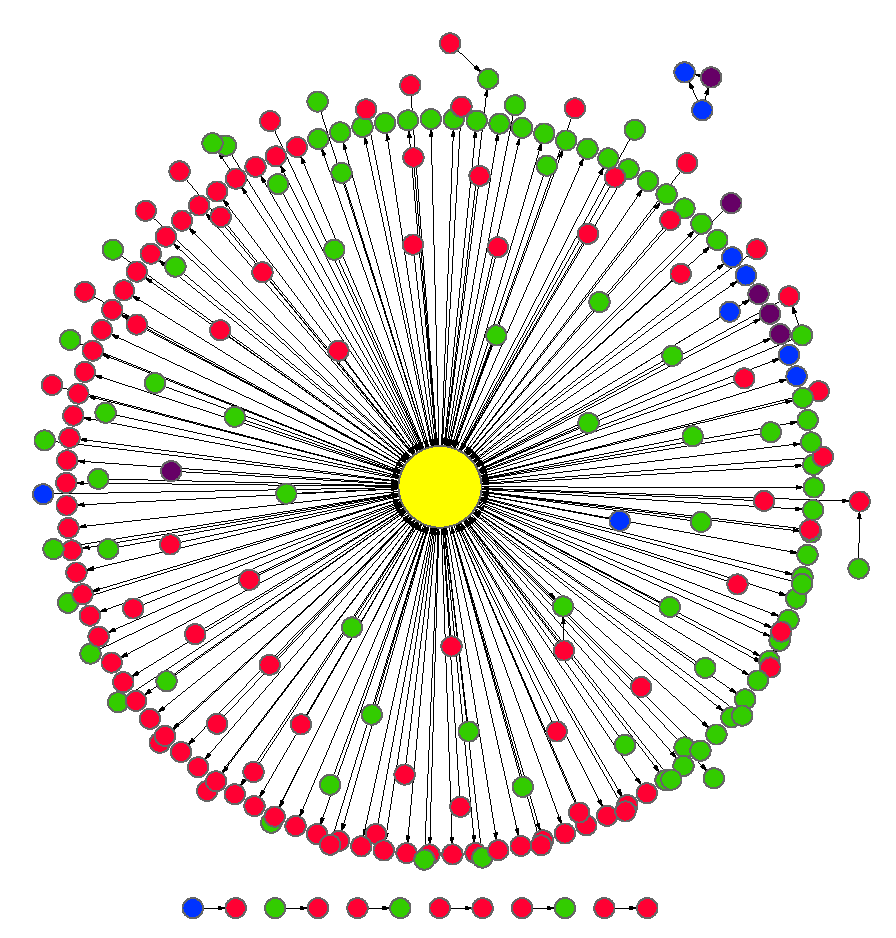
\includegraphics[scale=1.0]{images/component-metagraph-8.pdf}
  \caption{Struktur der starken Zusammenhangskomponenten bis zur
    Grösse 6 (rot = Grösse 6-10, grün = Grösse 11-20, blau = Grösse
    21-30, violett = Grösse $>= 31$, gelb = MSCC)}
  \label{fig:komponenten-struktur}
\end{figure}

Foobar bla bla bla.

\subsection{Communities}
\label{sec:result-communities}

Die Zerlegung des gerichteten Graphen mit dem Algorithmus von Rosval
et al. lieferte keine verwertbaren Ergebnisse. Zwar wurde eine
Zerlegung in 2869 Partitionen berechnet. Allerdings gilt f\"ur die
grosse Mehrzahl dieser Knotenmengen, dass der durch sie induzierte
Teilgraph \"uberhaupt keine Kanten hat. Nur f\"ur ca. 160 Partitionen
hat der jeweils induzierte Teilgraph Kanten, in allen F\"allen
allerdings sehr wenige (zwischen 1 und 104 f\"ur eine Partition der
Gr\"osse 682). Dass die Knoten einer Partition in allen F\"allen so
gut wie keine interne Vernetzung haben und damit der Definition von
Communities absolut nicht entsprechen, ist ein klarer Hinweis, dass
die berechnete Zerlegung die tats\"achliche modulare Struktur des
Graphen nicht sinnvoll wiedergibt. Dass der Graph in der Tat eine
ausgepr\"agte modulare Struktur hat, zeigen die anhand des
ungerichteten Graphen berechneten Zerlegungen, die auch unter
inhaltlichen Gesichtspunkten Sinn ergeben. Diese Struktur kann sich
auch nicht erst durch die Reduzierung des gerichteten auf einen
ungerichteten Graphen ergeben. Die berechnete Zerlegung mit etlichen
grossen Partitionen ohne interne Vernetzung ist in keinem Fall ein
sinnvolles Ergebnis eines Community-Algorithmus und spricht daher
f\"ur eine fehlerhafte Berechnung. Ob diese allerdings auf Fehler in
der verwendeten Implementierung der Autoren
\footnote{http://www.tp.umu.se/~rosvall/code.html} oder auf Fehler im
Algorithmus zur\"uckgeht, ist nicht bekannt.

F\"ur die restlichen Methoden wurde der Graph auf einen ungerichteten
Graphen reduziert. Dazu wurde jede einzelne gerichtete Kante in eine
ungerichte Kante umgewandelt. Aus dem gerichteten Graphen mit XXX
Kanten ergab sich so ein ungerichteter Graph mit 295425 Kanten.

F\"ur die COPRA-Berechnung wurden -- wie in \cite{Gregory2010}
vorgeschlagen -- Berechnungen mit unterschiedlichen Werten $v$
durchgef\"uhrt, um den ``besten'' Wert im Sinne der Modularity zu
ermitteln. Dabei ergaben sich mit steigender maximaler \"Uberlappung
$v$ nur bis $v\le 3$ steigende Modularity-Werte, dar\"uber hinaus
fielen sie kontinuierlich ab. Deshalb wurde die Berechnung mit $v=3$
verwendet. Die dort berechneten Modularity-Werte hatten eine geringe
Standardabweichung von 0,003. Dieses Ergebnis kommt unerwartet. In
\cite{Gregory2010} ergaben sich f\"ur ein PGP-Web-of-Trust-Netzwerk
mit 10680 Knoten bis zu $v=9$ ansteigende Modularity-Werte. Das
(lokale) Maximum bei geringem $v$ f\"ur das hier verwendete Netzwerk
k\"onnte darauf hinweisen, dass seine Community-Struktur keine
signifikante \"Uberlappung aufweist. Ein weiterer Hinweis darauf ist,
dass die Einf\"uhrung der \"Uberlappung mit $v=3$ gegen\"uber der
nicht \"uberlappenden Berechnung mit $v=1$ f\"ur die Modularity
(Tabelle \ref{tab:mod-result}) keinen signifikanten Anstieg
brachte. Auch die Zuordnung zu Gruppen bzw. Keysigning-Parties
(Tabelle \ref{tab:assign}) und die Verteilung der Gr\"osse der
Communities (Abbildungen \ref{fig:comsize-copra} und
\ref{fig:comsize-copra1}) \"ahneln sich weitgehend. Alternativ
k\"onnte dieses Ergebnis allerdings auch in einem nicht-optimalen
Verhalten des Algorithmus begr\"undet liegen.

\begin{figure}[t]
  \centering
  \subfloat[]{\label{fig:comsize-copra1} 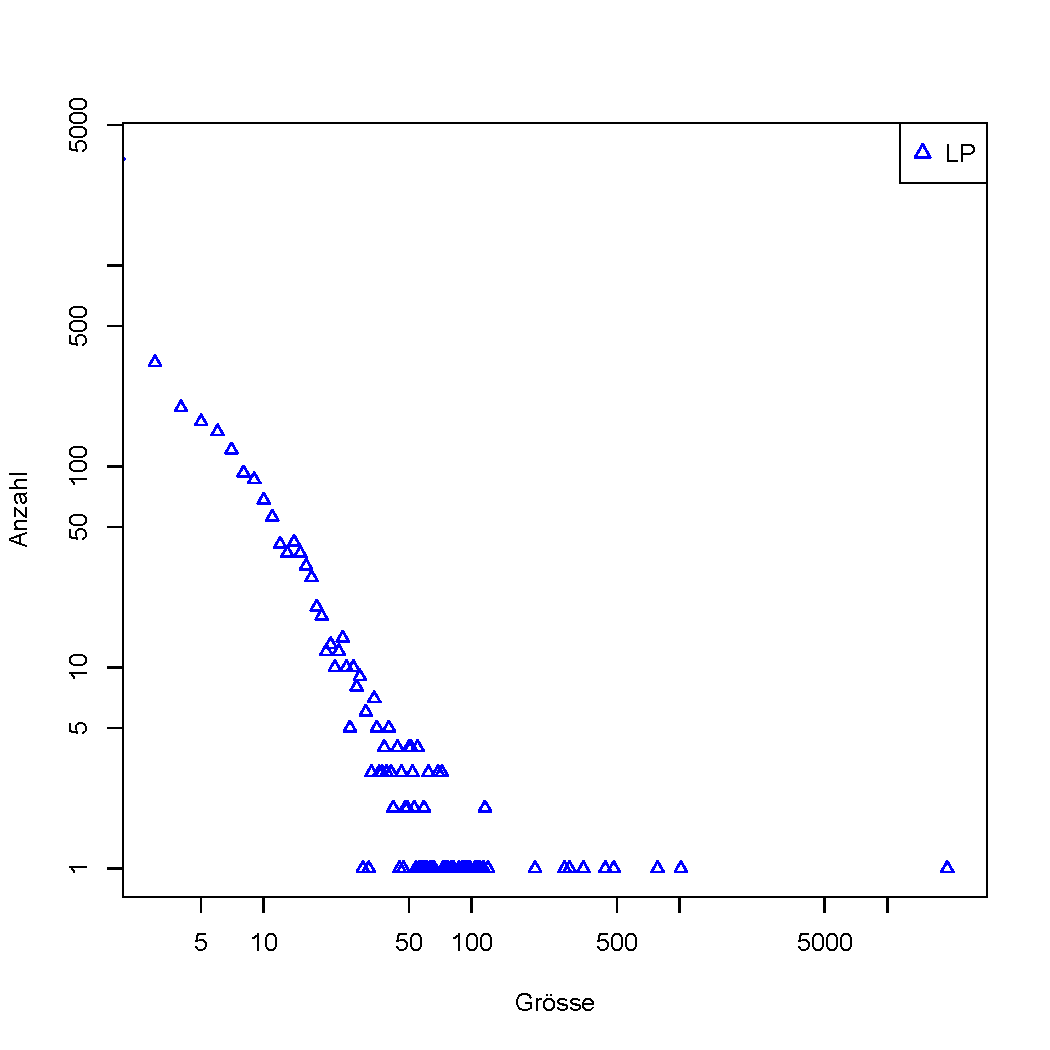
\includegraphics[scale=0.45]{images/community-size-dist_copra1.pdf}}
  \subfloat[]{\label{fig:comsize-copra} 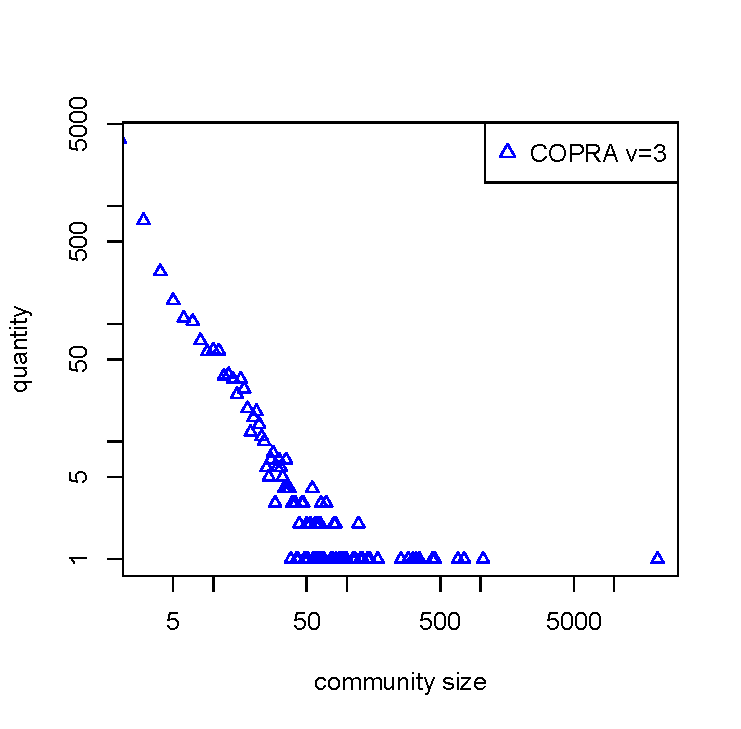
\includegraphics[scale=0.45]{images/community-size-dist_copra.pdf}} \\
  \subfloat[]{\label{fig:comsize-bl2} 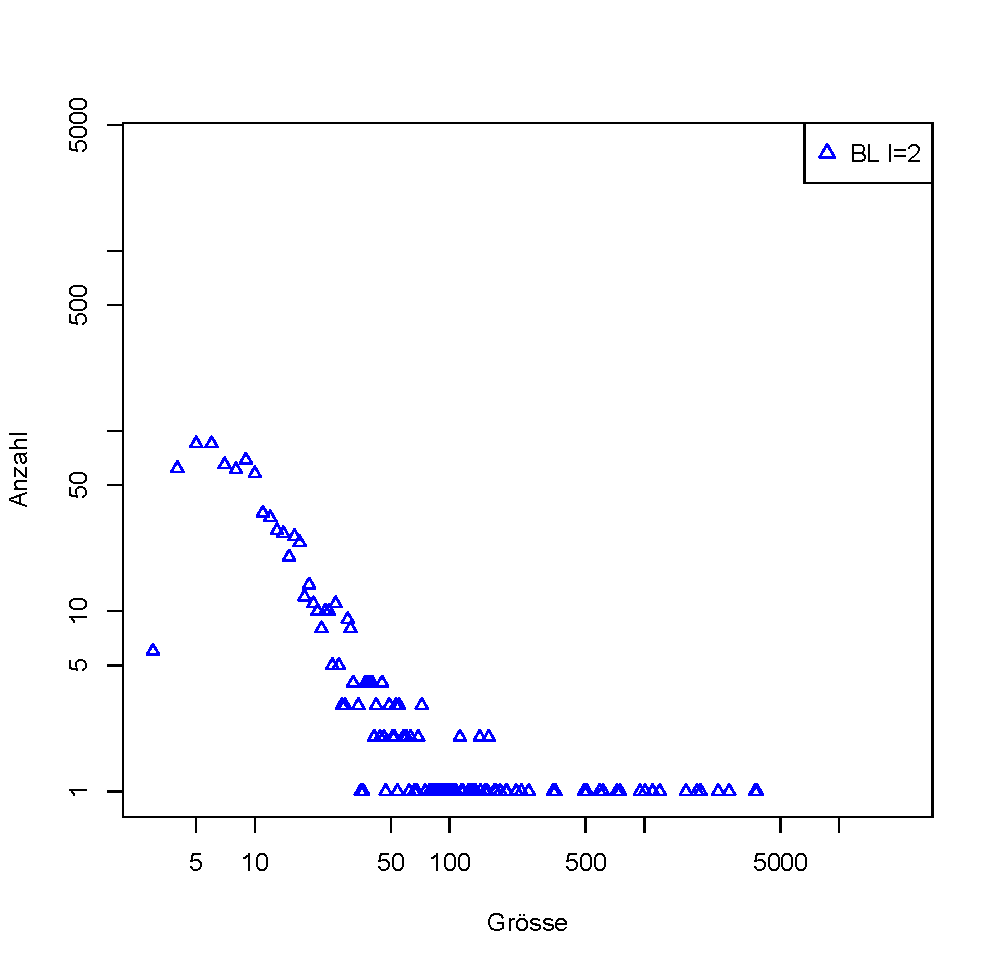
\includegraphics[scale=0.45]{images/community-size-dist_bl2.pdf}} 
  \subfloat[]{\label{fig:comsize-bl5} 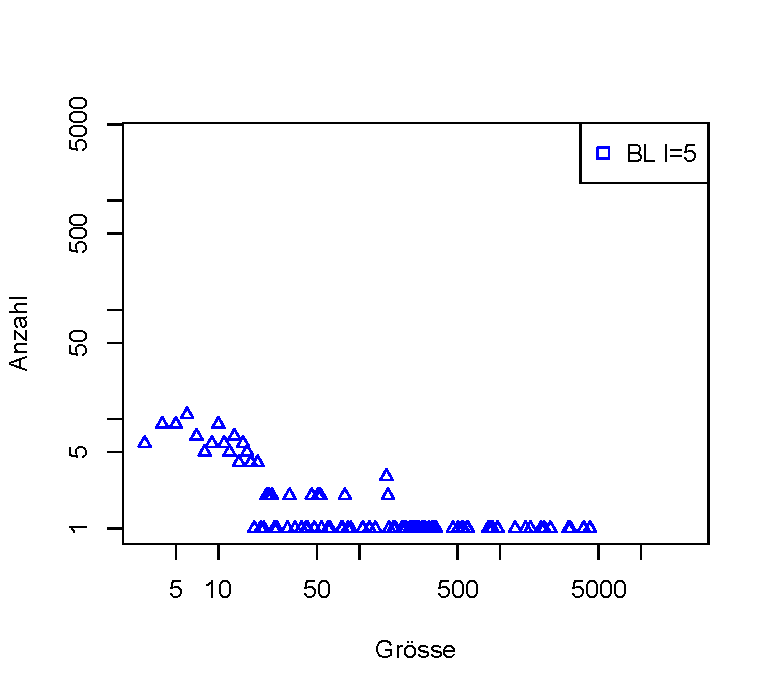
\includegraphics[scale=0.45]{images/community-size-dist_bl5.pdf}} 
  \caption{Gr\"ossenverteilung der Communities}
  \label{fig:comsizedist}
\end{figure}

F\"ur den Algorithmus von Blondel et al. zeigt sich zun\"achst ein
deutlich h\"oherer Modularity-Wert als f\"ur Fastmod. Dieses Ergebnis
gibt also die reine Struktur des Graphen deutlich besser wieder.  Wie
in Abschnitt
\ref{ch:Grundlagen:sec:Netzwerkanalyse:subsec:Communities}
beschrieben, verl\"auft der Algorithmus von Blondel et al. iterativ in
Phasen, in denen jeweils zuerst Knoten einer benachbarten Community
zugeordnet werden, wenn sich dadurch ein Modularity-Gewinn erzielen
l\"asst, und dann die Knoten dieser so entstandenen Communities zu
Knoten in einem neuen Netzwerk verschmolzen werden. Hier werden die
Ergebnisse der Phasen $l=2$ und der letzten Phase $l=5$
betrachtet. F\"ur $l=5$ ergab sich die h\"ochste
Modularity. Allerdings sticht hier die sehr kleine Anzahl von
Communities heraus, die wiederum vergleichsweise gross sein
m\"ussen. Gegen\"uber dem Ergebnis der Phase 2 ergibt sich eine
relativ kleine Steigerung der Modularity, die mit einem erheblichen
Verlust an \emph{Aufl\"osung} erkauft wird\footnote{Die Zerlegungen
  der Phasen 3 und 4 unterschieden sich nur geringf\"ugig von der
  Zerlegung der Phase 5}. Aus Abbildung \ref{fig:comsize-bl2} und
\ref{fig:comsize-bl5} geht hervor, dass diese Reduktion der Anzahl im
Wesentlichen auf das Reduzieren sehr kleiner Communities
zur\"uckgeht. Da der Algorithmus von Blondel et al. genauso wie
Fastmod mittels einer (lokalen) Optimierung der Modularity arbeitet,
k\"onnte dieses Ph\"anomen auf das in der Literatur beschriebene
Aufl\"osungslimit der Modularity-Funktion (bspw. \cite{Fortunato2007}
\cite{Good2009}) zur\"uckzuf\"uhren sein. Es scheint fraglich, ob die
in Relation zur Gr\"osse des Graphen sehr geringe Zahl von 186
Communities die Struktur des Graphen (in Bezug auf die inhaltliche
Analyse) ad\"aquat wiedergibt.

\begin{figure}[ht]
  \centering
  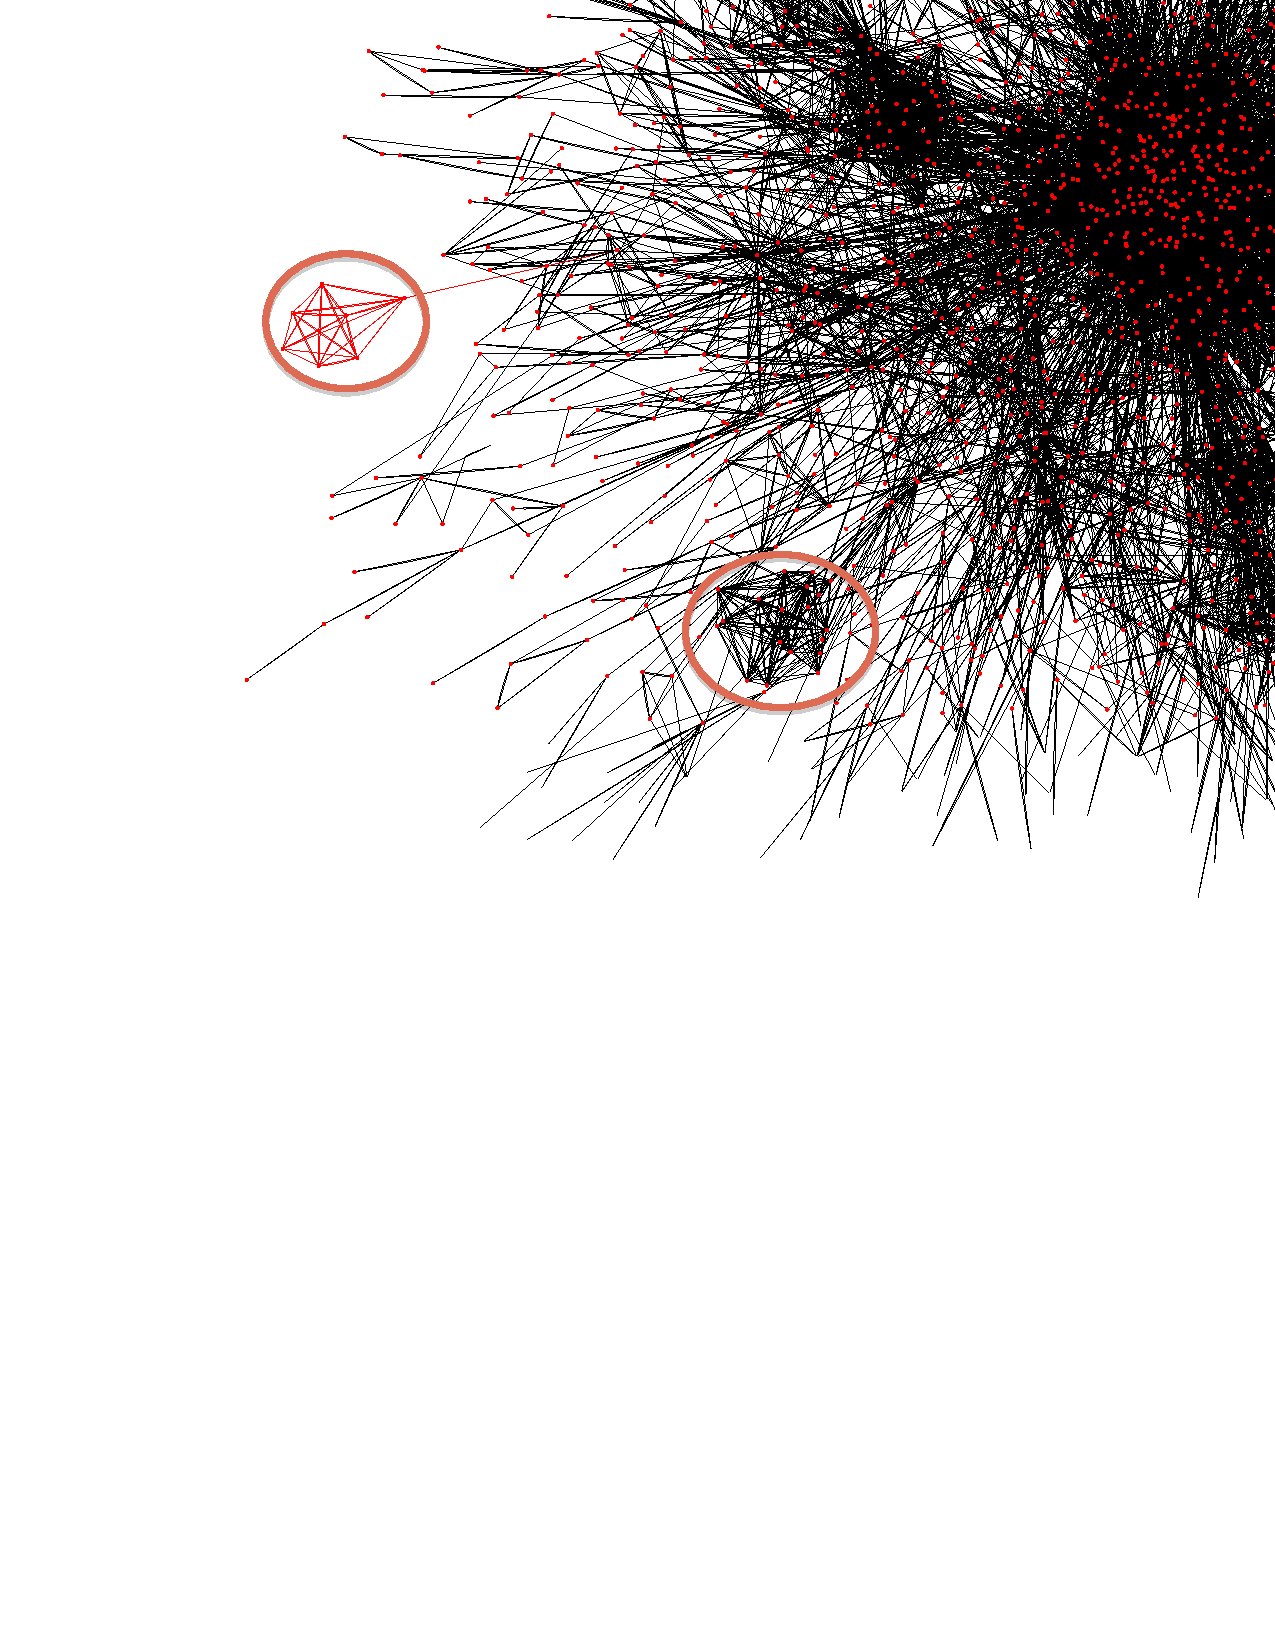
\includegraphics[scale=0.7]{images/blondel-l5-com-c3a5eaab680984b123037897b0be74bf-edit.pdf}
  \caption{Community mit modularen Untereinheiten (Gr\"osse 2271,
    Blondel ($l=5$), Force-directed Layout)}
  \label{fig:large-modular}
\end{figure}

Abbildung \ref{fig:large-modular} illustriert dies anhand einer
Community aus der Zerlegung des Algorithmus von Blondel et al. mit
$l=5$, die klar abgegrenzte Untereinheiten enth\"alt, die intuitiv
wieder eigenst\"andige Communities darstellen.


Abbildung \ref{fig:large-community-modular} illustriert die begrenzte
Qualit\"at der Fast-Modularity-Zerlegung, die sich im vergleichweise
niedrigen Modularity-Wert niederschl\"agt. In der Zeichnung des
induzierten Teilgraphen einer grossen Community sind etliche dicht
gezeichnete Zusammenballungen von Knoten zu sehen, die nur wenige
Kanten nach aussen haben. Diese k\"onnen als Community-artige
Strukturen interpretiert werden. Zwar kann argumentiert werden, dass
die Zeichnung die Struktur des Teilgraphen nicht notwendigerweise
sinnvoll wiedergibt, dass also die dichten Teilbereiche in der
Zeichnung nur Artefakte der Zeichenmethode darstellen. Allerdings
zeigt Noack, dass starke \"Ubereinstimmungen zwischen einer
energieoptimalen Einbettung eines Graphen in die Ebene nach der
Force-directed-Methode und einer Partitionierung eines Graphen mit
optimaler Modularity bestehen \cite{Noack2009}. Es scheint daher
gerechtfertigt, eine Zeichnung eines Graphen (Force-directed) mit
markanten dichten Bereichen als Indiz f\"ur eine modulare Struktur
dieses Graphen zu betrachten.


\begin{table}[t]
  \centering
  \footnotesize
  \begin{tabular}{l|c|c|c}
    Algorithmus & Modularity & Communities &
    Enthaltene Knoten \\
    \hline
    FM & 0,596 & 552 & 44611 \\
    \hline
    BL ($l=2$)& 0,701 & 936 & 44934 \\
    BL ($l=5$)& 0,710 & 186 & 44934 \\
    \hline
    COPRA ($v=1$) & (0,780) & 1421 & 42205 \\
    COPRA ($v=3$) & (0,786) & 1354 & --- \\

  \end{tabular}
  \caption{Modularity-Werte, Anzahl der Communities mit mehr als 3
    Knoten sowie die Anzahl der insgesamt in diesen Communities (>3) enthaltenen
    Knoten 
    f\"ur die Algorithmen Fast-Modularity (FM), Label-Propagation
    (LP), Blondel et al. (BL) auf Level 2 und 5 sowie COPRA. Die
    Modularity-Werte f\"ur COPRA entsprechen der Modularity-Definition
    f\"ur \"uberlappende Zerlegungen nach \cite{Nicosia2009} und k\"onnen mit den anderen
    Werten nicht verglichen werden.}
  \label{tab:mod-result}
\end{table}

Aus Tabelle \ref{tab:mod-result} geht hervor, dass sich -- zumindest
im Fall von Fastmod und Blondel et al. -- fast alle Knoten des Graphen
in einer Community wiederfinden, die mindestens die Gr\"osse 4 hat. In
Abschnitt \ref{sec:result-allg-merkm-des} wurde gezeigt, dass ein
erheblicher Anteil der Knoten einen sehr geringen Grad von 1 oder 2
hat. Da solche Knoten mangels Kanten nicht selbst eine dichte
Vernetzung herstellen k\"onnen, m\"ussen sie Mitglied in Communities
sein, in denen Knoten mit h\"oherem Grad sowohl die interne Vernetzung
der Community als auch die Vernetzung der Community mit anderen
erzeugen. COPRA scheint hingegen dazu tendieren, deutlich mehr Knoten
in Communities sehr kleiner Gr\"osse mit 3 oder weniger
unterzubringen. Dieses Verhalten k\"onnte dazu f\"uhren, dass die
Aussagekraft der Zerlegung in Bezug auf die realen Communities
geschw\"acht wird, wenn viele Knoten auf diese Art abgespalten werden.

Gegen\"uber der COPRA-Zerlegung mit $v=1$ zeigt die Zerlegung mit
$v=3$ eine deutlich gr\"ossere Anzahl von Communities der Gr\"osse 3
und 4. Abgesehen davon \"ahneln sich die Gr\"ossenverteilungen aber
weitgehend. Beide enthalten eine charakteristische sehr grosse
Community mit ca. 19000 bzw. ca. 21000 Mitgliedern. Demgegen\"uber
bietet die Blondel-Zerlegung mit $l=2$ eine deutlich geringere Anzahl
solcher sehr kleiner Communities, daf\"ur aber eine h\"ohrere Zahl
mittlerer (mehr als 100 Mitglieder) und insbesondere eine h\"ohere
Zahl sehr grosser (zwischen 500 und 5000 Mitglieder).

Blondel ist insgesamt vom Resolution limit gestraft
(wg. mod. maximierung) und bietet daher nicht die notwendige
aufloesung, um communities besser inhaltlich analysieren zu koennen.

Der insgesamt recht hohe Modularity-Wert weist darauf hin, dass der
Graph in der Tat eine ausgepr\"agte modulare Struktur hat, wie dies
von einem sozialen Netzwerk erwartet wird.

\begin{table}[t]
  \centering
  \footnotesize
  \begin{tabular}{l|c|c|c|c|c}
    Algorithmus & TLD-S & TLD-M & SLD-S & SLD-M & SIG \\
    \hline
    FM & 293 (53\%) & 247 (44\%) & 56 (10\%) & 154 (27\%) & 128
    (23\%) \\
    \hline
    BL ($l=2$) & 499 (53\%) & 417 (45\%) & 41 (4\%) & 254 (27\%) & 115 (12\%) \\
    BL ($l=5$) & 85 (47\%) & 85 (47\%) & 15 (8\%) & 38 (21\%) & 26 (14\%) \\
    \hline
    COPRA ($v=1$) & 824 (58\%) & 564 (40\%) & 178 (13\%) & 429 (30\%)
    & 572 (40\%) \\
    COPRA ($v=3$) & 792 (58\%) & 525 (38\%) & 187 (14\%) & 425 (31\%) & 555
    (41\%)
  \end{tabular}
  \caption{SLD-TLD-Zuweisung, TIME-CORR}
  \label{tab:assign}
\end{table}

Aus Tabelle \ref{tab:assign} geht hervor, dass f\"ur alle Zerlegungen
fast alle Communities einer Top-Level-Domain zuordnenbar sind oder von
einer TLD dominiert werden. Werden die generischen Top-Level-Domains
(gTLD: com, org, net, info, ...) abgezogen, verbleiben im Fall von COPRA
noch 519 (38\%) Communities, die einer TLD (und damit einer
\emph{Country-Coded TLD (ccTLD)}) zugeordnet werden k\"onnen und 315
(23\%), die von einer ccTLD dominiert werden. F\"ur die anderen
Zerlegungen ergeben sich \"ahnliche Werte. Damit ist immerhin etwa die
H\"alfte der Communities einem Land zuordnenbar. F\"ur die von einer
gTLD dominierten Communities ergeben Stichproben, dass sich die
Teilnehmer der meisten dieser Communities anhand der Namen zumindest
einem Sprachraum zuweisen lassen.

Dieses Ergebnis ist naheliegend. Wie in Abschnitt
\ref{sec:community-analyse} dargelegt, wird davon ausgegangen, dass
ein wesentlicher Faktor, der das Zustandekommen von Signaturen
beeinflusst, die sozialen Kontakte einer Person sind. Es ist weiterhin
naheliegend, dass sich diese sozialen Kontakte unter anderem aufgrund
von Sprachbarrieren und der r\"aumlichen N\"ahe haupts\"achlich im
Rahmen eines Landes ergeben. Beispielsweise ist f\"ur eine aus
Finnland stammende Person anzunehmen, dass die Mehrzahl ihrer Freunde,
Bekannten, Gesch\"aftspartner und sonstigen Kontakte wieder Finnen
sind.

Zwar k\"onnte argumentiert werden, dass das Internet die geographische
bzw. nationale Beschr\"ankung sozialer Kontakte aufhebt. Allerdings
spielt die geographische N\"ahe eine wichtige Rolle im
Signaturprozess. Die verbreitete Prozedur f\"ur das Signieren eines
Schl\"ussels setzt ein direktes pers\"onliches Treffen der
Signierenden voraus (siehe Abschnitt \ref{sec:sozi-komp-des}). Es ist
anzunehmen, dass die \"uberwiegende Mehrheit der PGP-Benutzer die
meiste Zeit in einem Land und damit in einem geographisch
eingegrenzten Bereich verbleibt. Damit kommen f\"ur diese Mehrheit
\"uberwiegend nur Bewohner des gleichen Landes als Signaturpartner in
Frage. Als Mechanismen f\"ur die internationale Vernetzung kommen dann
etwa internationale Konferenzen in Frage. Nur ein sehr kleiner Teil
der PGP-Benutzer d\"urfte die notwendige internationale Mobilit\"at
aufweisen, so dass sich seine Signaturen nicht \"uberwiegend einem
geographischen Bereich bzw. einem Land zuweisen lassen.

Interessanter f\"ur die Fragestellung ist aber die Erkennung von
Keysigning-Parties und die Zuordnung zu Second-Level-Domains. 

\begin{figure}[th]
  \centering
  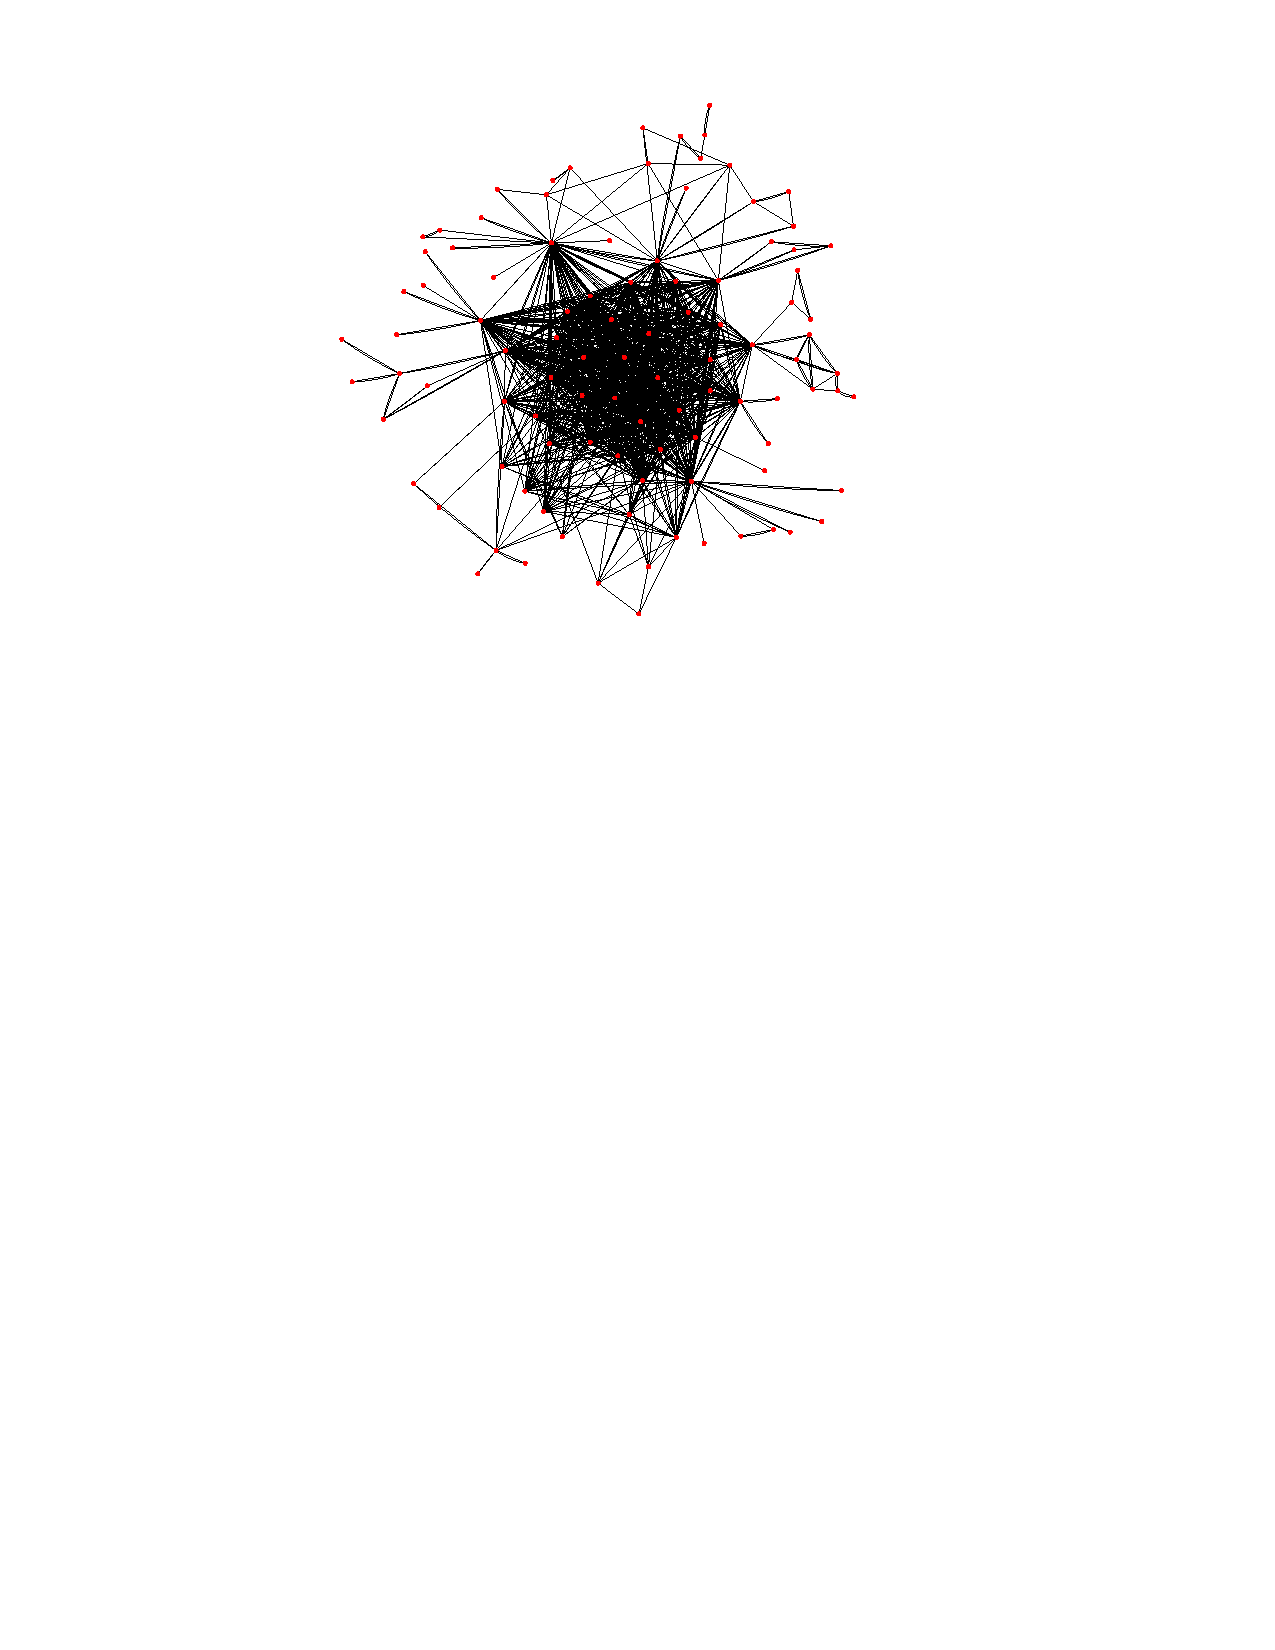
\includegraphics[scale=1.5]{images/subgraph-label-time-fa62cc57cd35e9f90b85435efc407ad5.pdf}
  \caption{Community mit zeitlicher Korrelation der Signaturen
    (Blondel ($l=5$),
    100 Knoten, 72\% der Signaturen innerhalb eines Monats)}
  \label{fig:time-corr-com-normal}
\end{figure}


\begin{figure}[th]
  \centering
  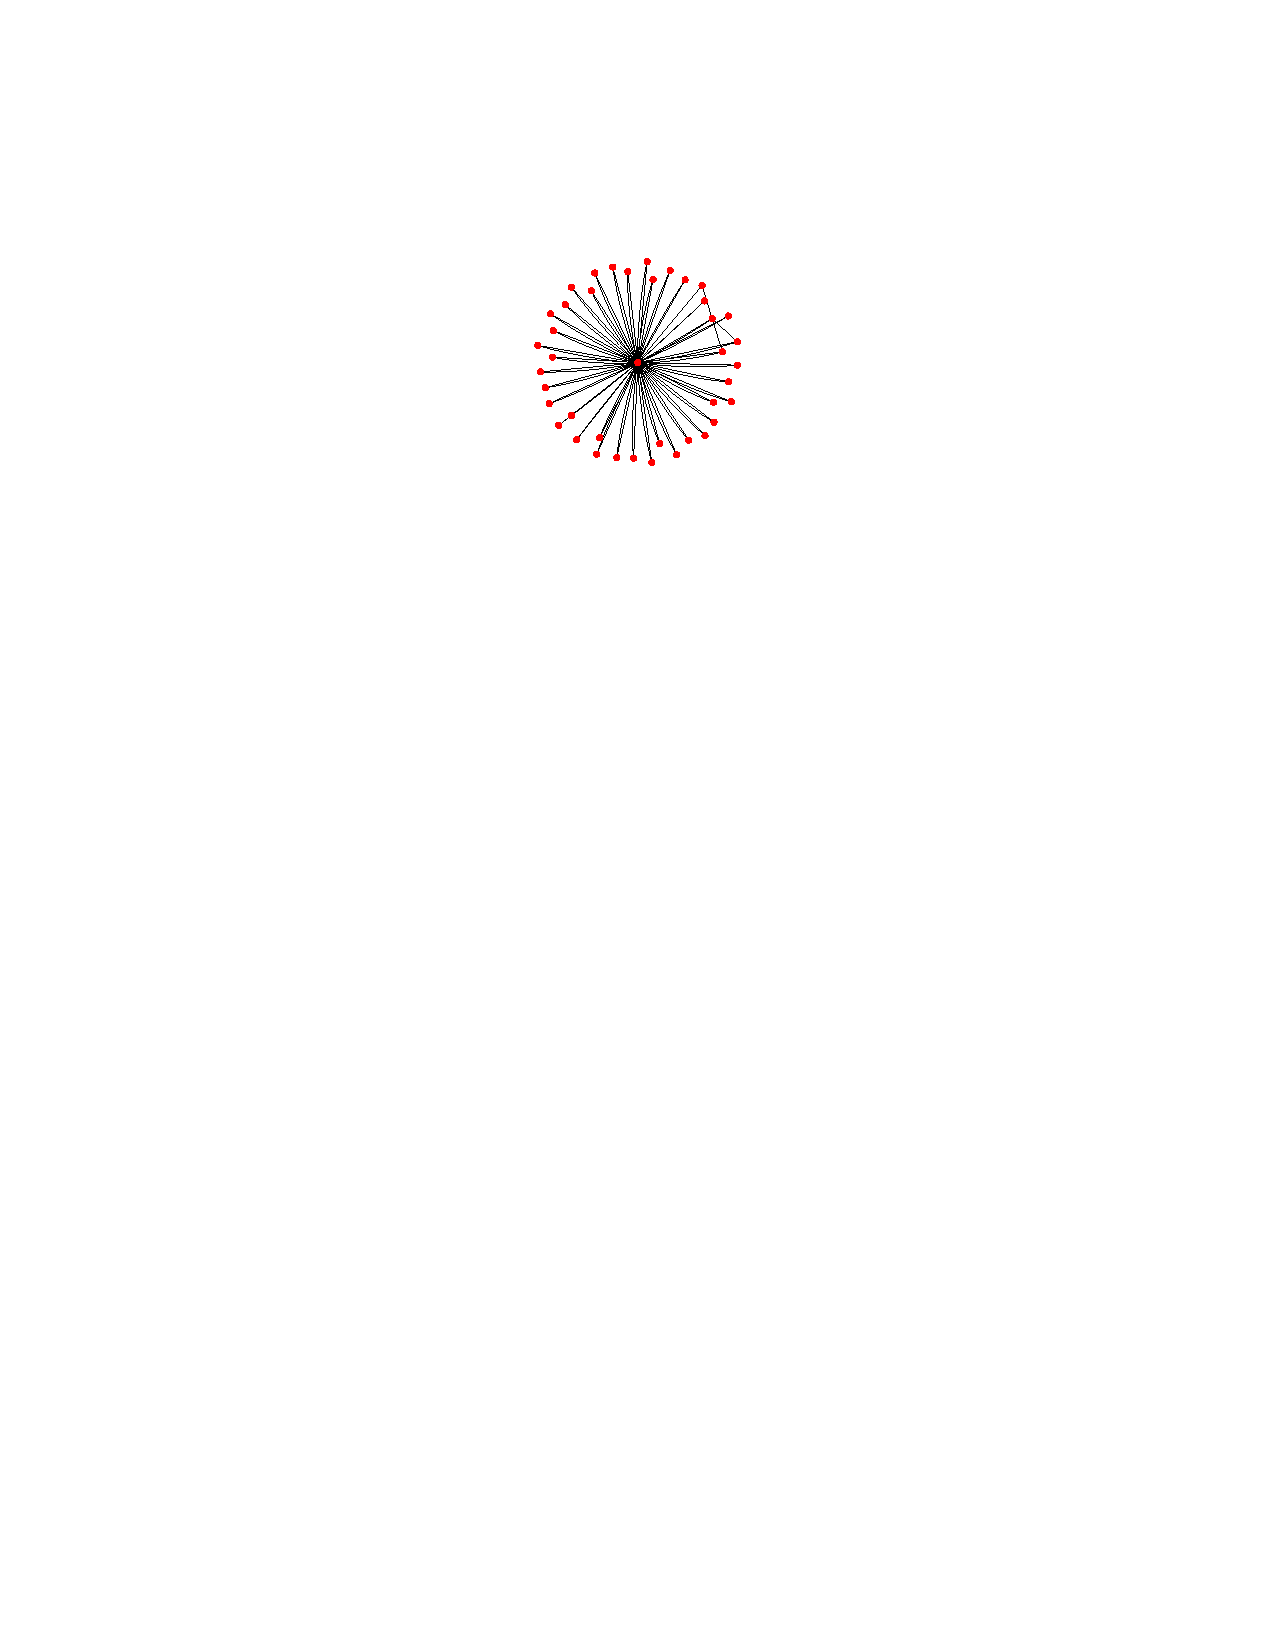
\includegraphics[scale=1.3]{images/label-subgraph-41-star-c222345bc5eb1f9eff80d58a81861974.pdf}
    \caption{Community mit zeitlicher Korrelation der Signaturen
      (Blondel ($l=5$),
      41 Knoten, 84 \% der Signaturen innerhalb eines Monats)}
  \label{fig:time-corr-com-star}
\end{figure}


Es stellt sich die Frage, ob die zeitliche Korrelation der Signaturen
in einer Community ein geeignetes Mittel ist, um Keysigning-Parties zu
erkennen. Neben dem zeitlichen Zusammenhang der Signaturen ist ein
weiteres Merkmal einer Keysigning-Party wie in
Ab. \ref{sec:sozi-komp-des} beschrieben, dass jeder Teilnehmer mit
(fast) jedem anderem Teilnehmer Signaturen austauscht, so dass sich
eine fast vollst\"andige Vermaschung -- fast eine Clique --
ergibt. Eine stichprobenartige Untersuchung in den Communities zeigt,
dass die meisten Communities mit zeitlicher Korrelation zumindest
teilweise dieses Merkmal zeigen. Abbildung
\ref{fig:time-corr-com-normal} zeigt ein Beispiel einer solchen
Community. Etwa die H\"alfte der Knoten ist in einer Fast-Clique
enthalten, deren Knoten mit (fast) allen anderen vernetzt sind. Dieser
innere Teil des Teilgraphen entspricht genau dem Bild, das als
Resultat einer Keysigning-Party erwartet wird. Auch wenn dies auf die
meisten der Communities mit zeitlicher Korrelation zutrifft, gibt es
auch Gegenbeispiele. Abbildung \ref{fig:time-corr-com-star} zeigt eine
Community, die zwar das Kriterium der zeitlichen Korrelation
erf\"ullt, ansonsten aber nichts mit dem erwarteten Bild einer KSP
gemein hat. Allerdings erf\"ullt der Teilgraph trotzdem das Kriterium
der Community, da die Knoten am Rand nur Signaturen zu dem zentralen
Knoten haben und damit die interne Kantendichte deutlich h\"oher ist
als die externe. Um solche Extremf\"alle auszuschliessen, ist als
zus\"atzliches Kriterium f\"ur die Erkennung von KSPs ein hoher
durchschnittlicher Grad der Knoten denkbar.


\begin{figure}[h]
  \centering
  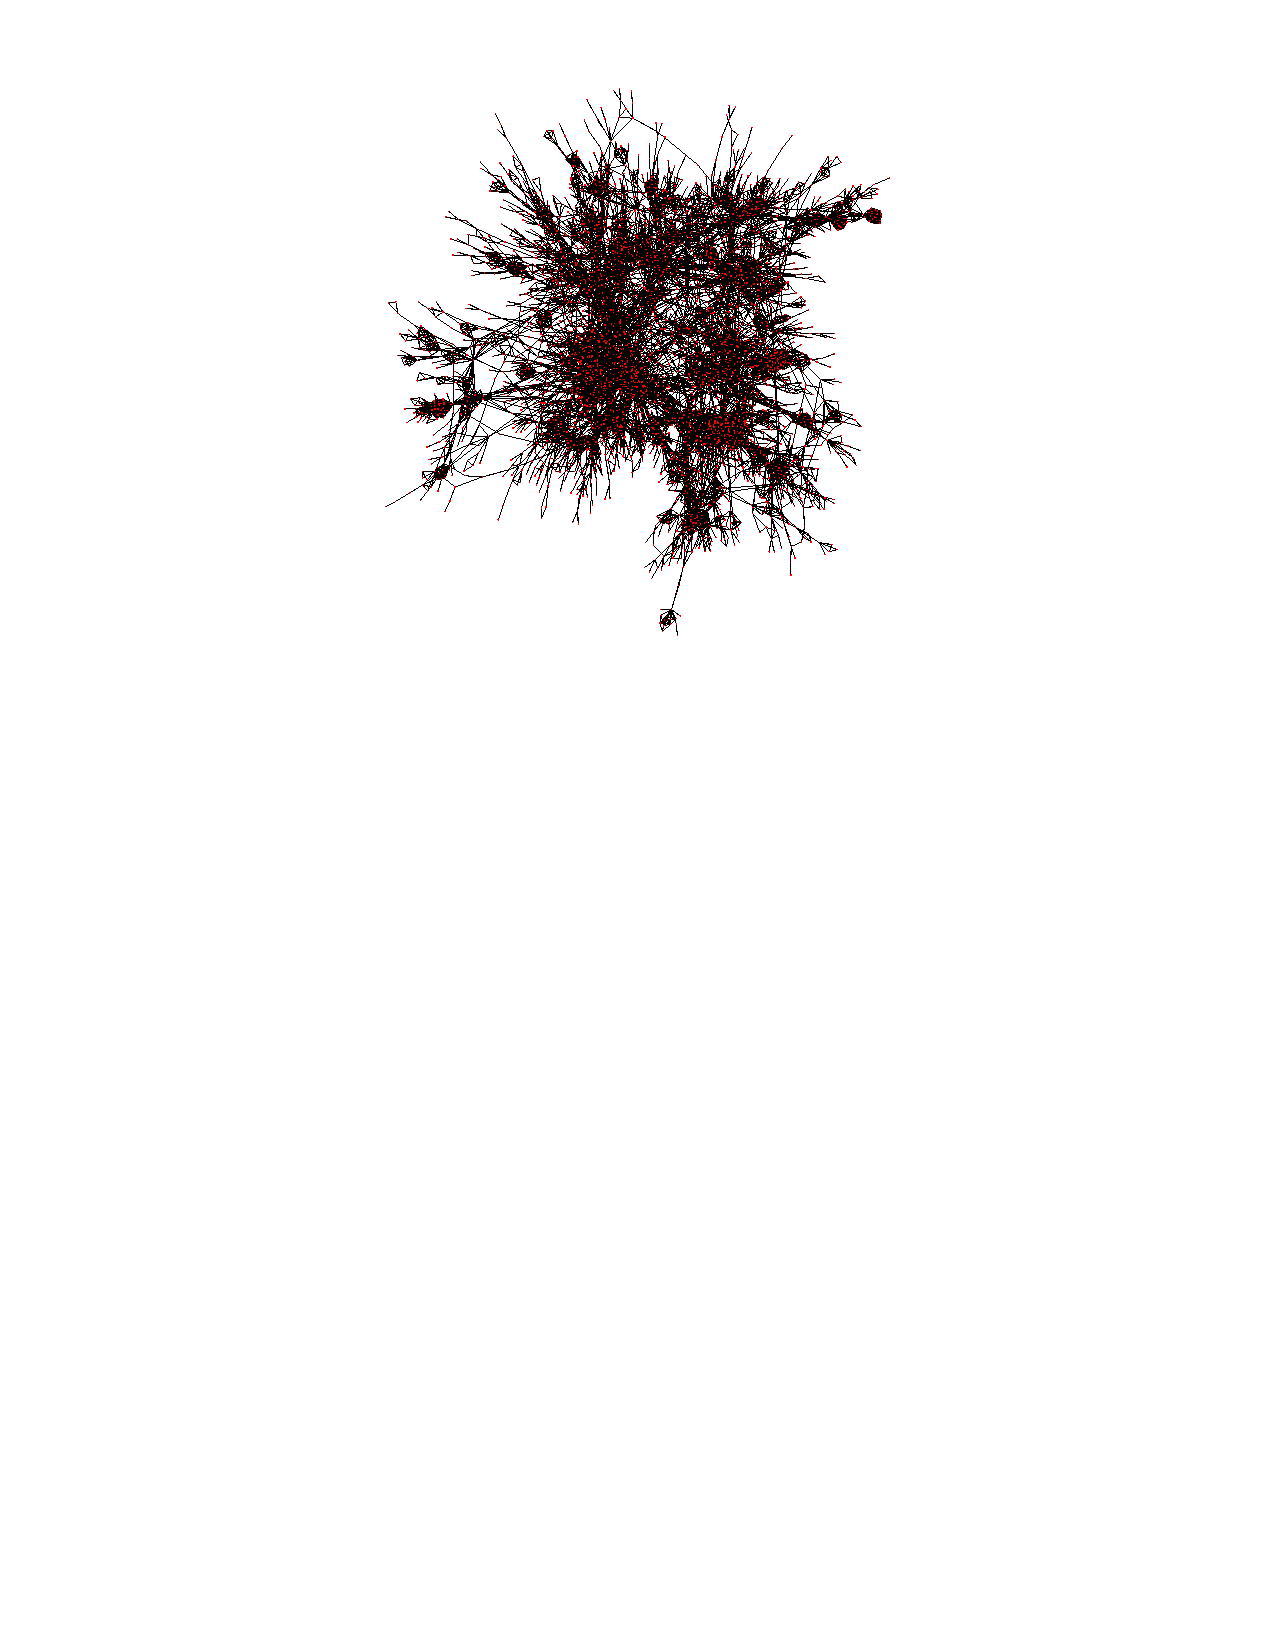
\includegraphics[scale=1.7]{images/fastmod-subgraph-large-modular-6525064ccab580a0b304a3620b197d7a.pdf}
  \caption{Grosse Community mit modularer Struktur (Berechnet mit
    Fast-Modularity, Force-directed layout)}
  \label{fig:large-community-modular}
\end{figure}
\begin{figure}[h]
  \centering
  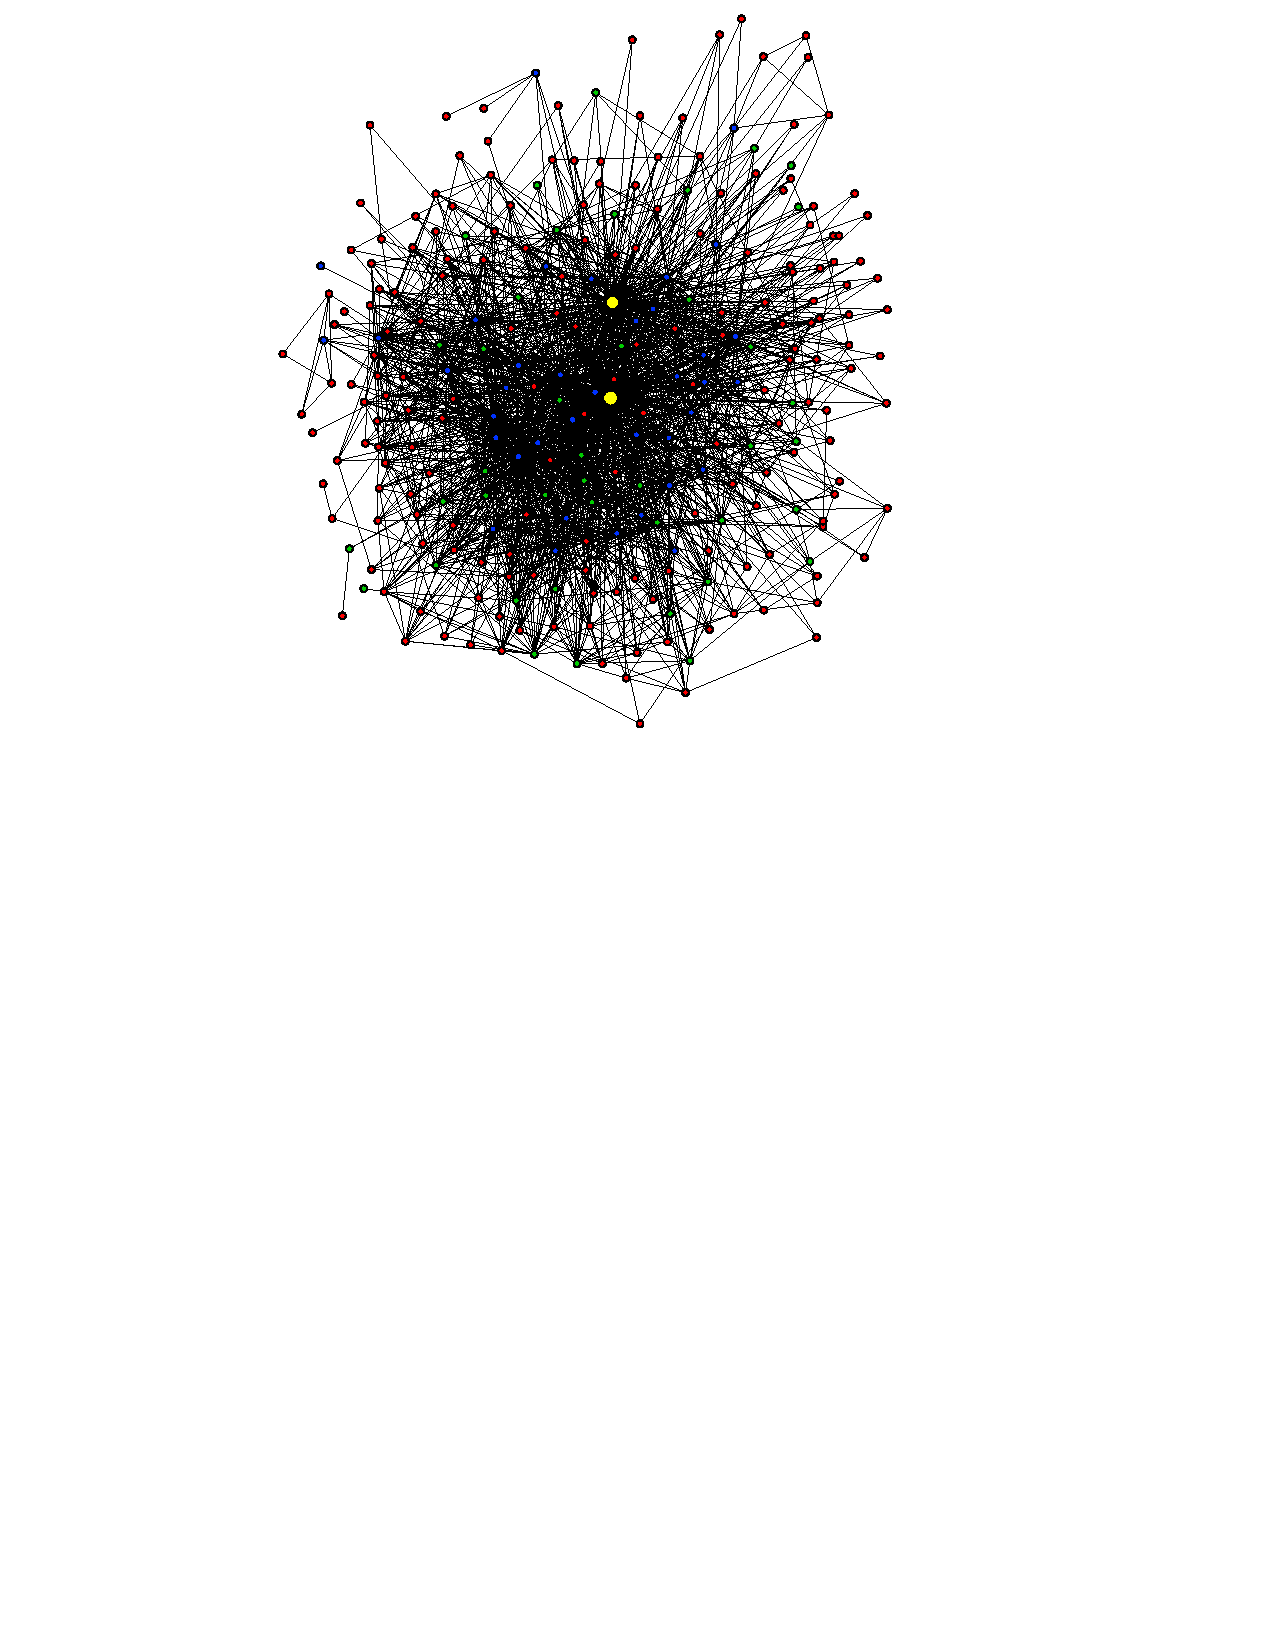
\includegraphics[scale=1.5]{images/label-prop-metagraph-20-narrow-cut.pdf}
  \caption{Struktur der Communities (Label-Propagation) (rot: Gr\"osse
    $<50$, gr\"un: Gr\"osse $<100$, blau: Gr\"osse < 1000, gelb:
    Gr\"osse > 1000).}
  \label{fig:metagraph-com-label}
\end{figure}


\begin{figure}[h]
  \centering
  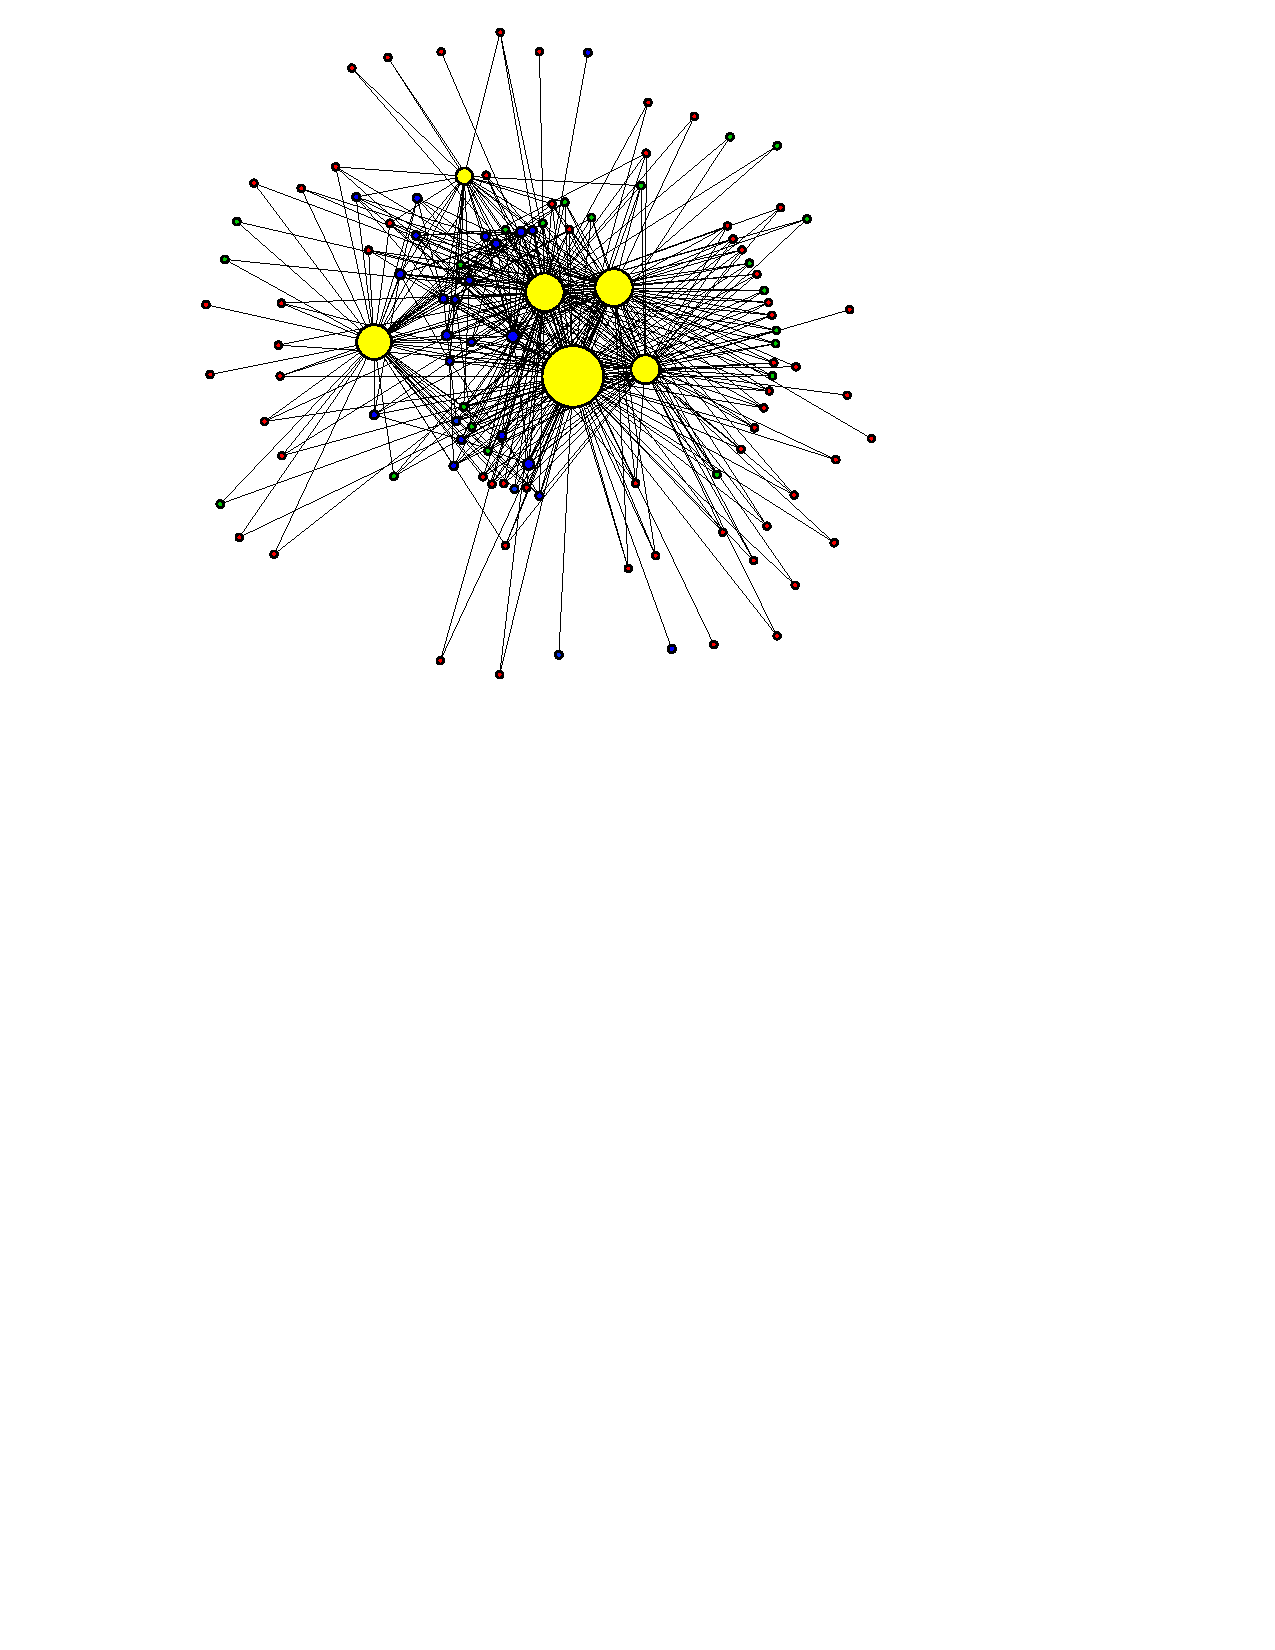
\includegraphics[scale=1.0]{images/fastmod-metagraph-20.pdf}
  \caption{Struktur der Communities (Fast Modularity) (Knotenf\"arbung
    wie in Abb.\ref{fig:metagraph-com-label})}
  \label{fig:metagraph-com-fastmod}
\end{figure}


%\begin{figure}[t]
%  \centering
%  \subfloat[]{\label{fig:tld-sure-copra1} 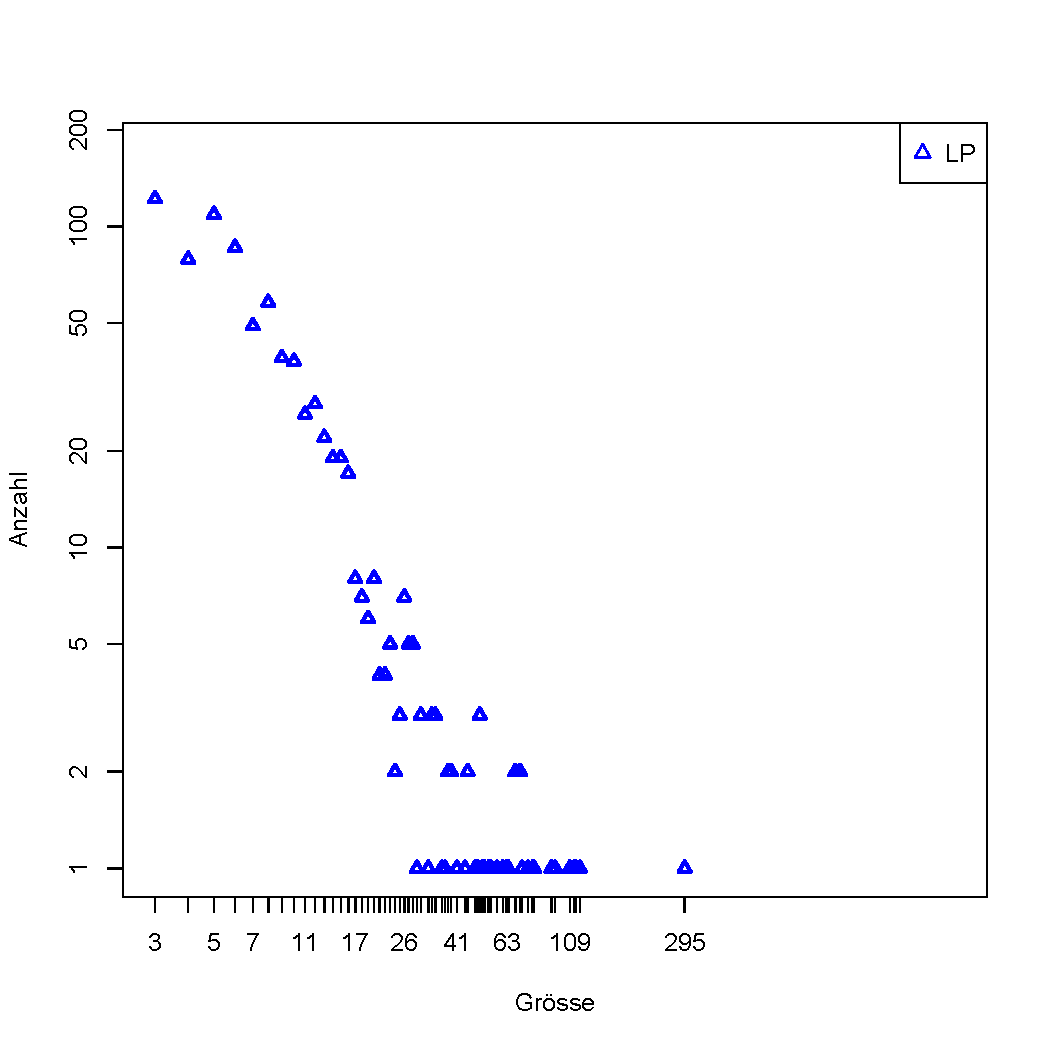
\includegraphics[scale=0.45]{images/tld-sure-ass_copra1.pdf}}
%  \subfloat[]{\label{fig:tld-sure-bl2} 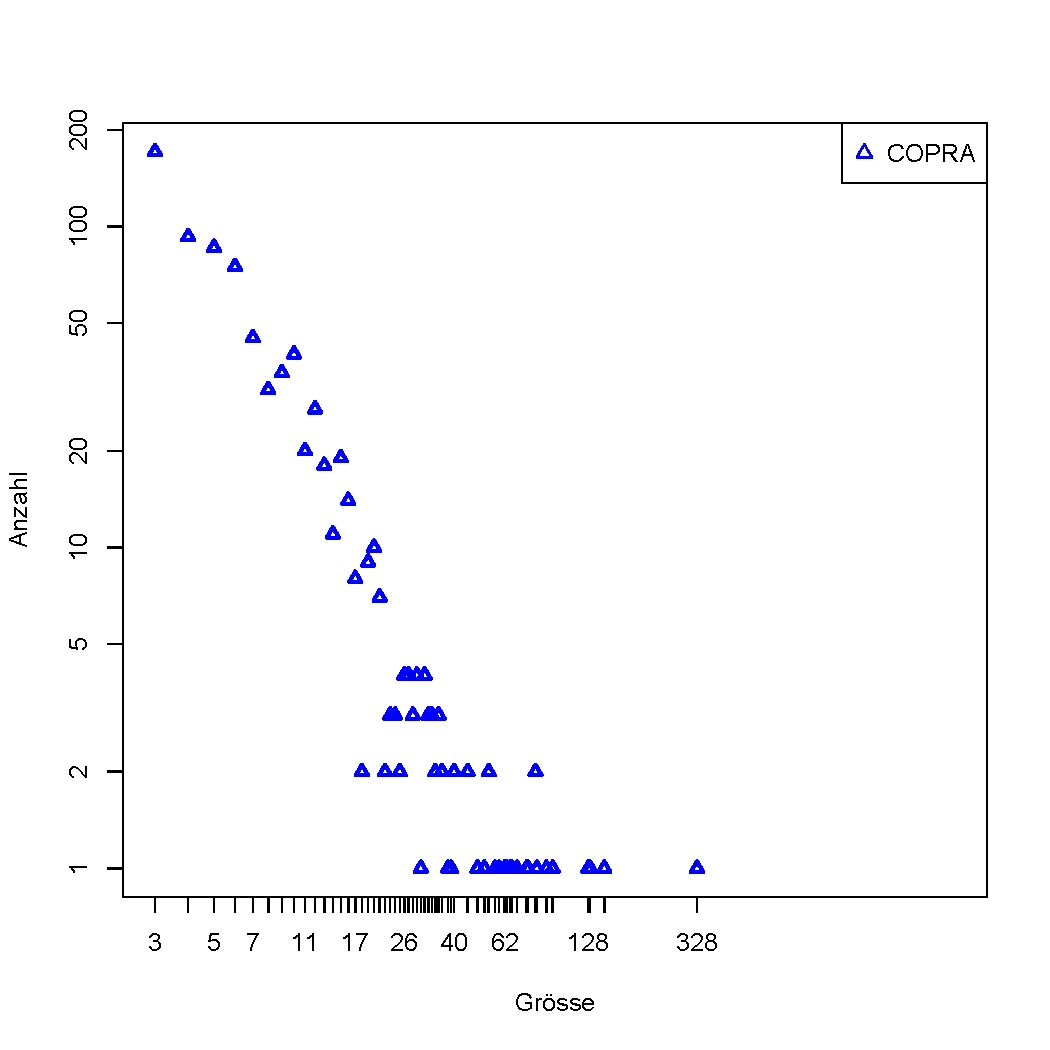
\includegraphics[scale=0.45]{images/tld-sure-ass_copra.pdf}}\\
%  \subfloat[]{\label{fig:tld-sure-bl5} 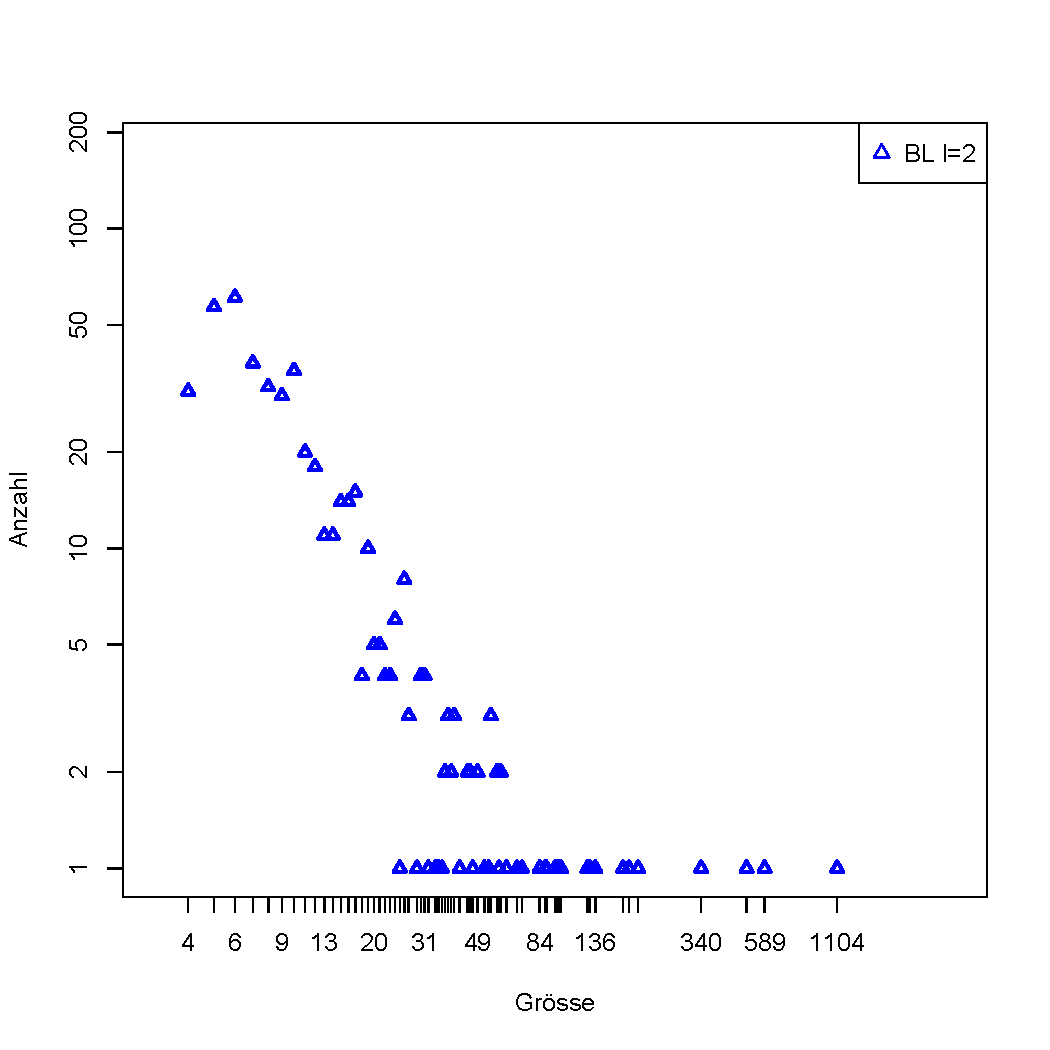
\includegraphics[scale=0.45]{images/tld-sure-ass_bl2.pdf}} 
%  \subfloat[]{\label{fig:tld-sure-copra} 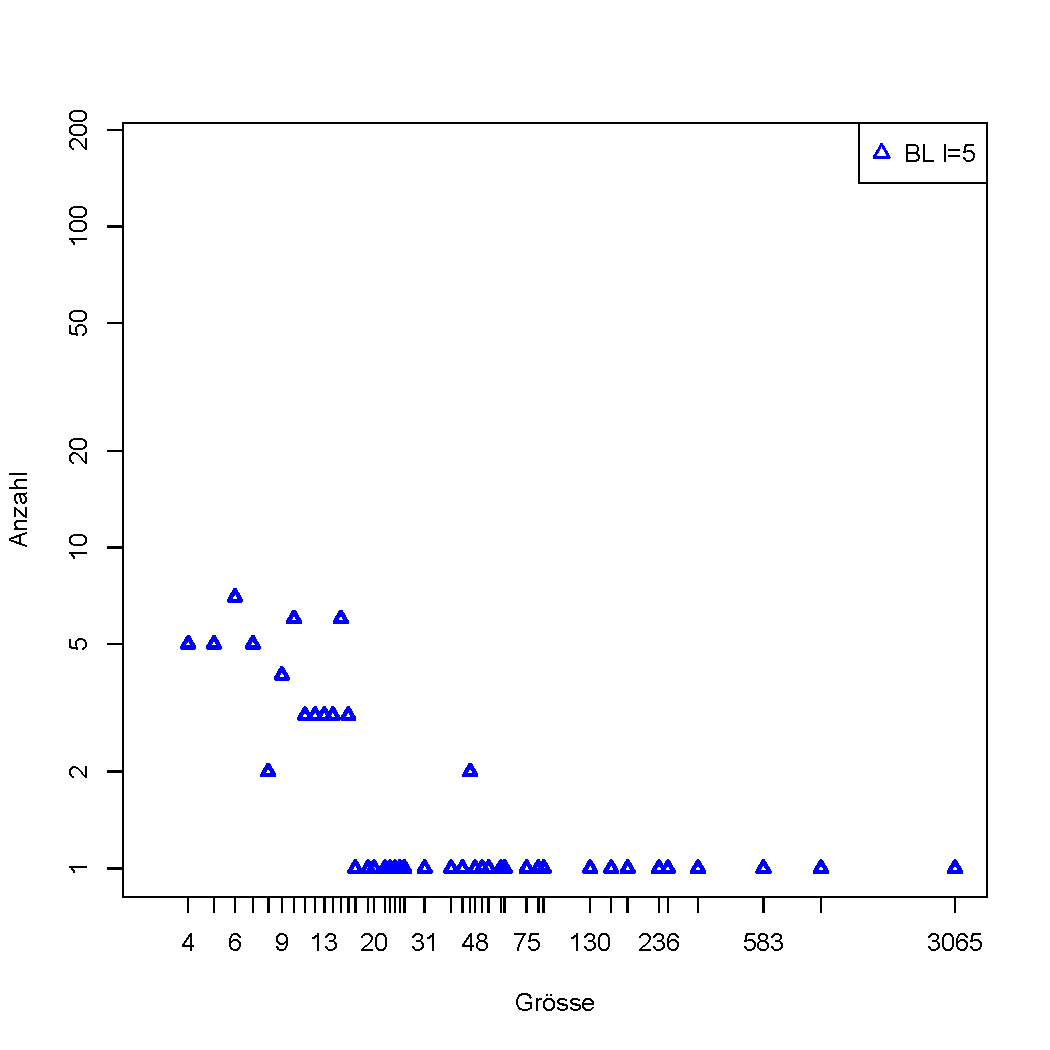
\includegraphics[scale=0.45]{images/tld-sure-ass_bl5.pdf}}
%  \caption{Zuweisung von Domains zu TLDs abh\"angig von der Community-Gr\"osse}
%  \label{fig:tld-suredist}
%\end{figure}

%\begin{figure}[t]
%  \centering
%  \subfloat[]{\label{fig:tld-maybe-copra1} 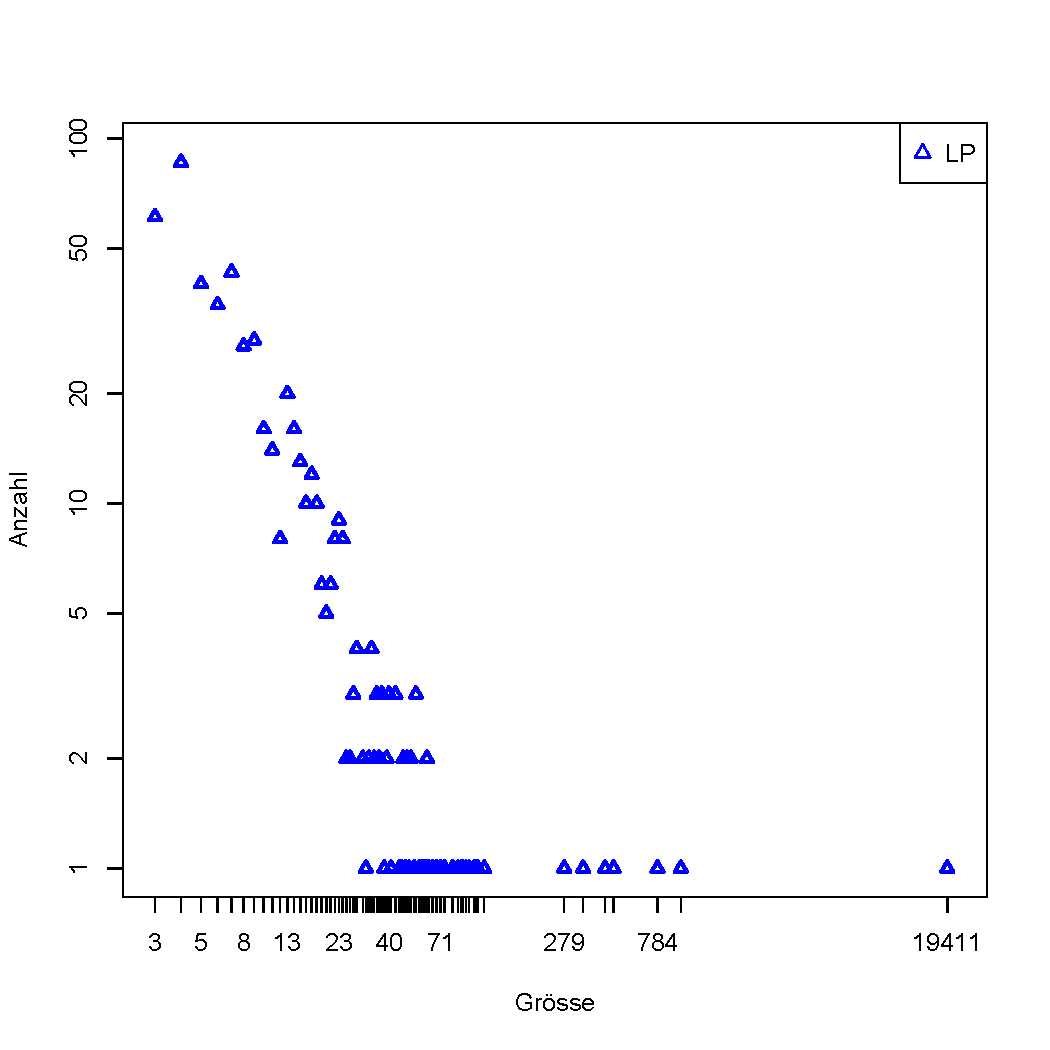
\includegraphics[scale=0.45]{images/tld-maybe-ass_copra1.pdf}}
%  \subfloat[]{\label{fig:tld-maybe-bl2} 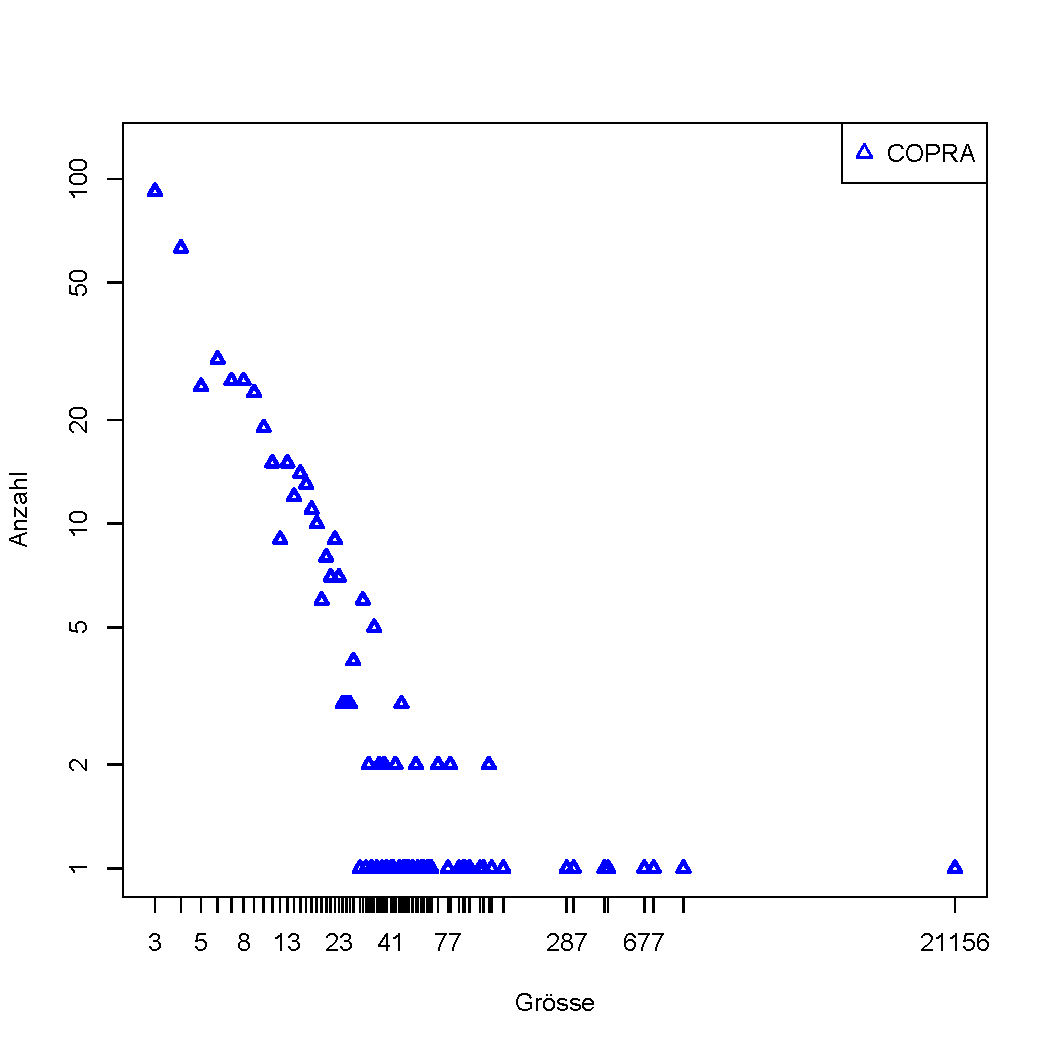
\includegraphics[scale=0.45]{images/tld-maybe-ass_copra.pdf}}\\
%  \subfloat[]{\label{fig:tld-maybe-bl5} 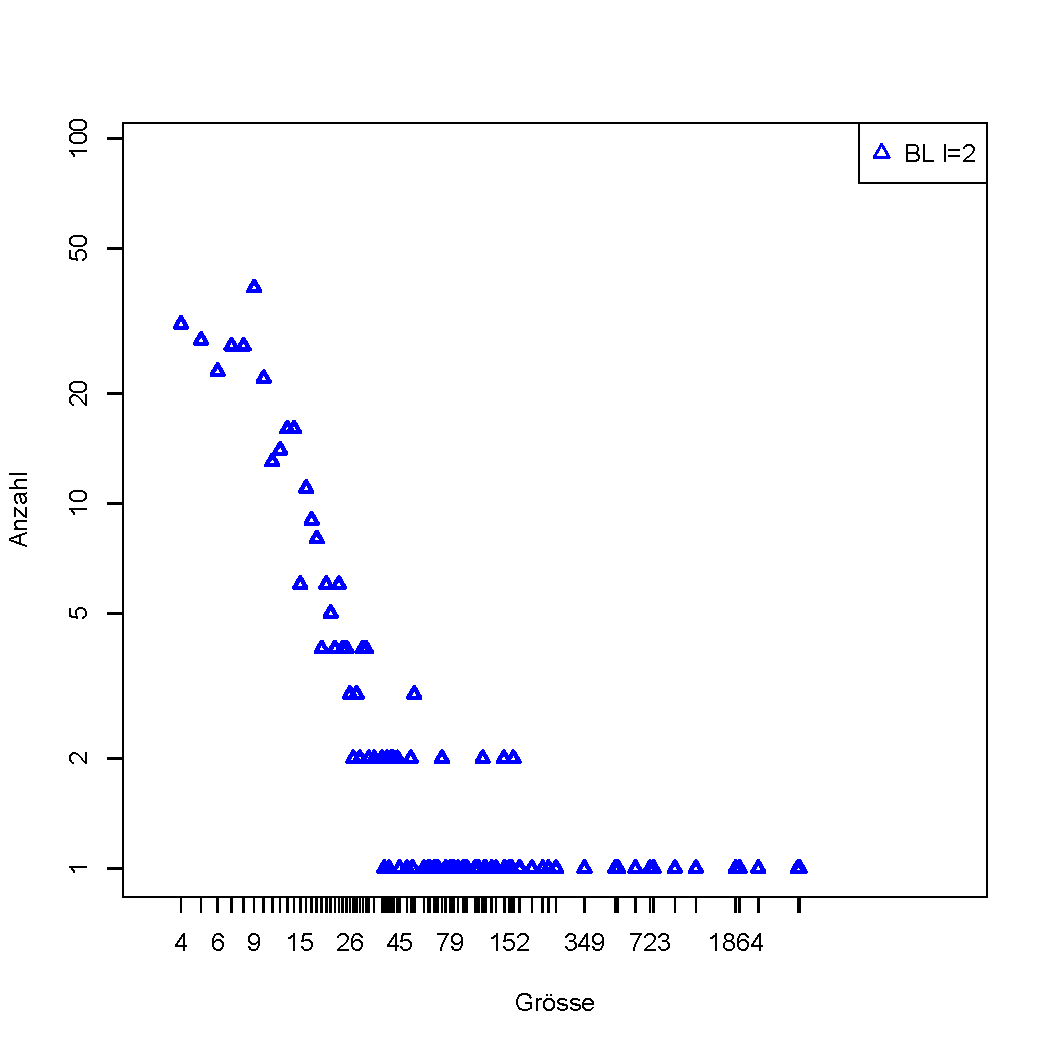
\includegraphics[scale=0.45]{images/tld-maybe-ass_bl2.pdf}} 
%  \subfloat[]{\label{fig:tld-maybe-copra} 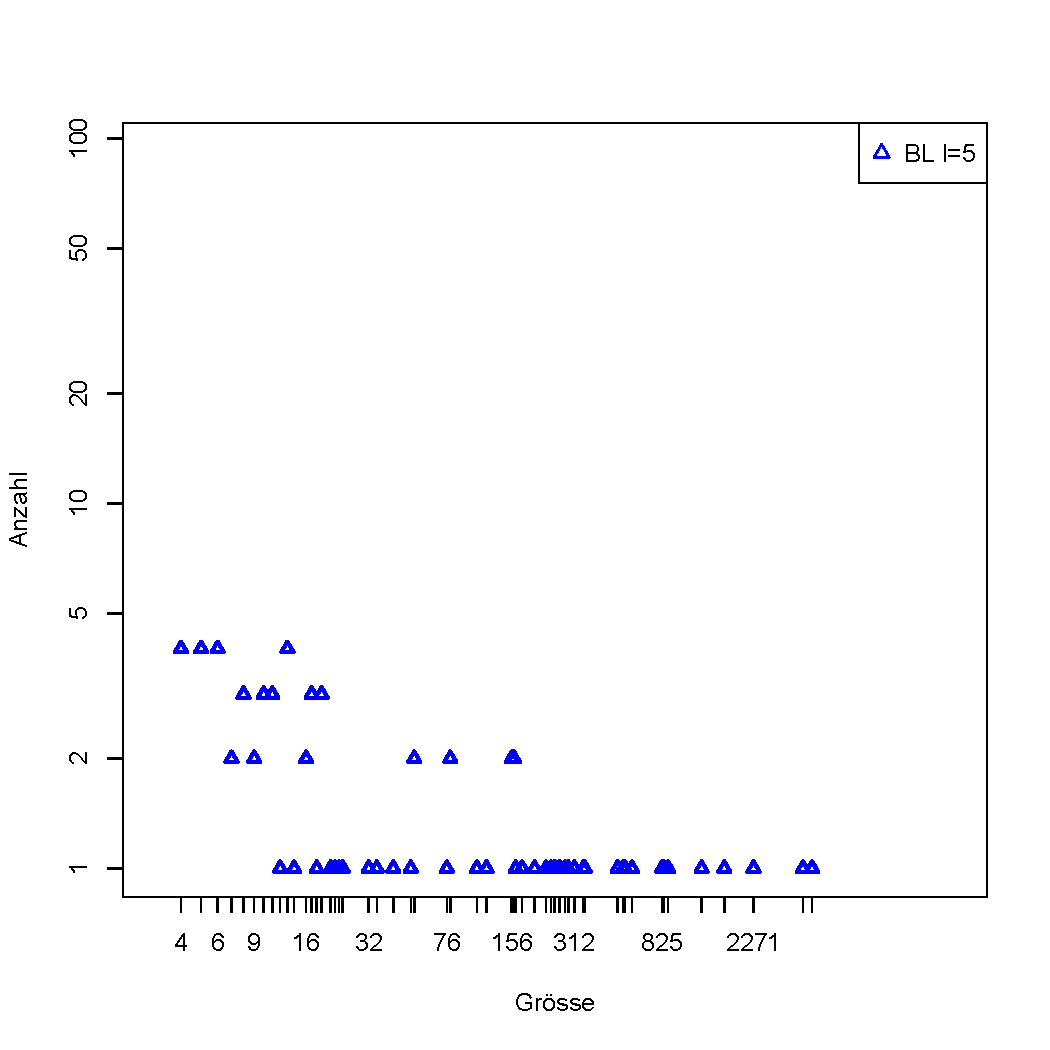
\includegraphics[scale=0.45]{images/tld-maybe-ass_bl5.pdf}}
%  \caption{Verteilung der Gr\"osse der von einer TLD dominierten Communities}
%  \label{fig:tld-maybedist}
%\end{figure}

\begin{figure}[t]
  \centering
  \subfloat[]{\label{fig:sld-sure-copra1} 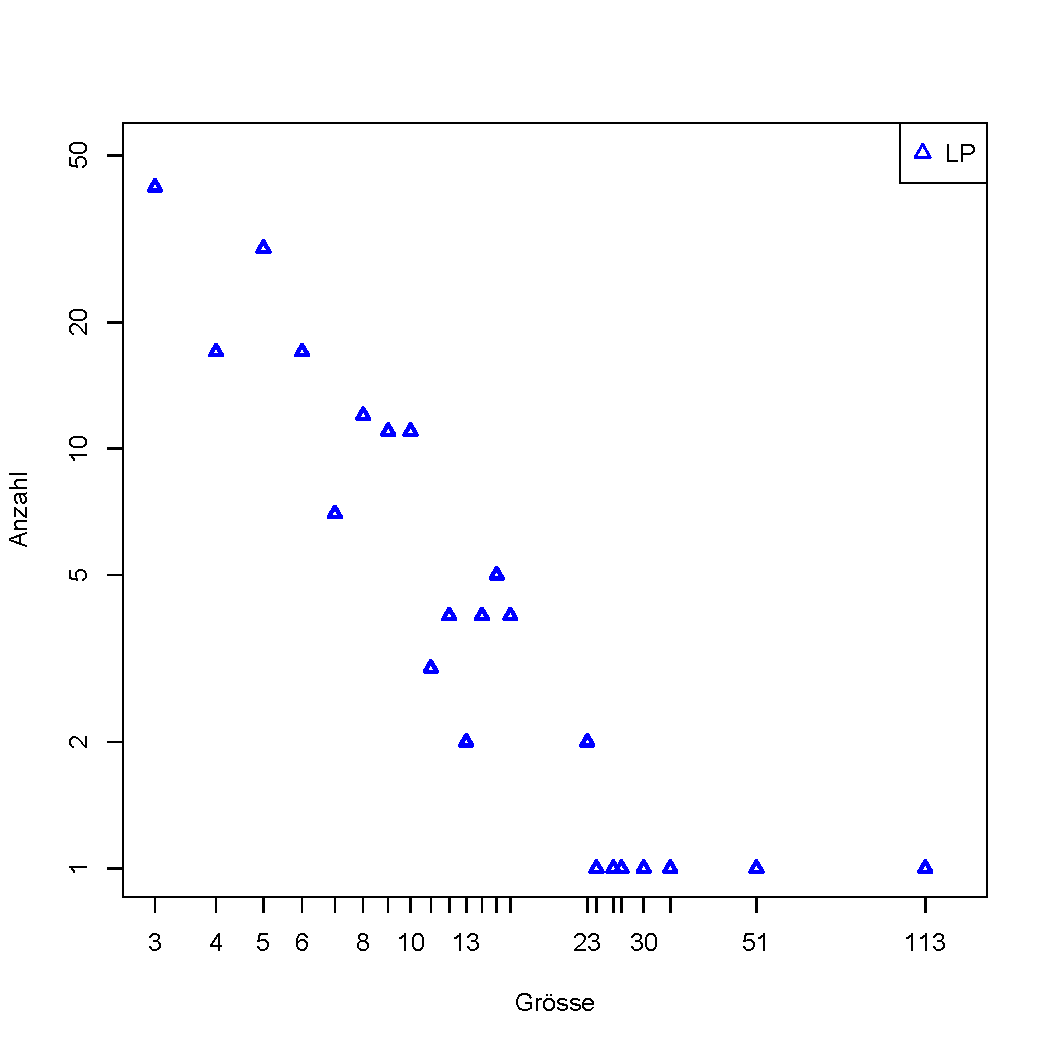
\includegraphics[scale=0.45]{images/sld-sure-ass_copra1.pdf}}
  \subfloat[]{\label{fig:sld-sure-bl2} 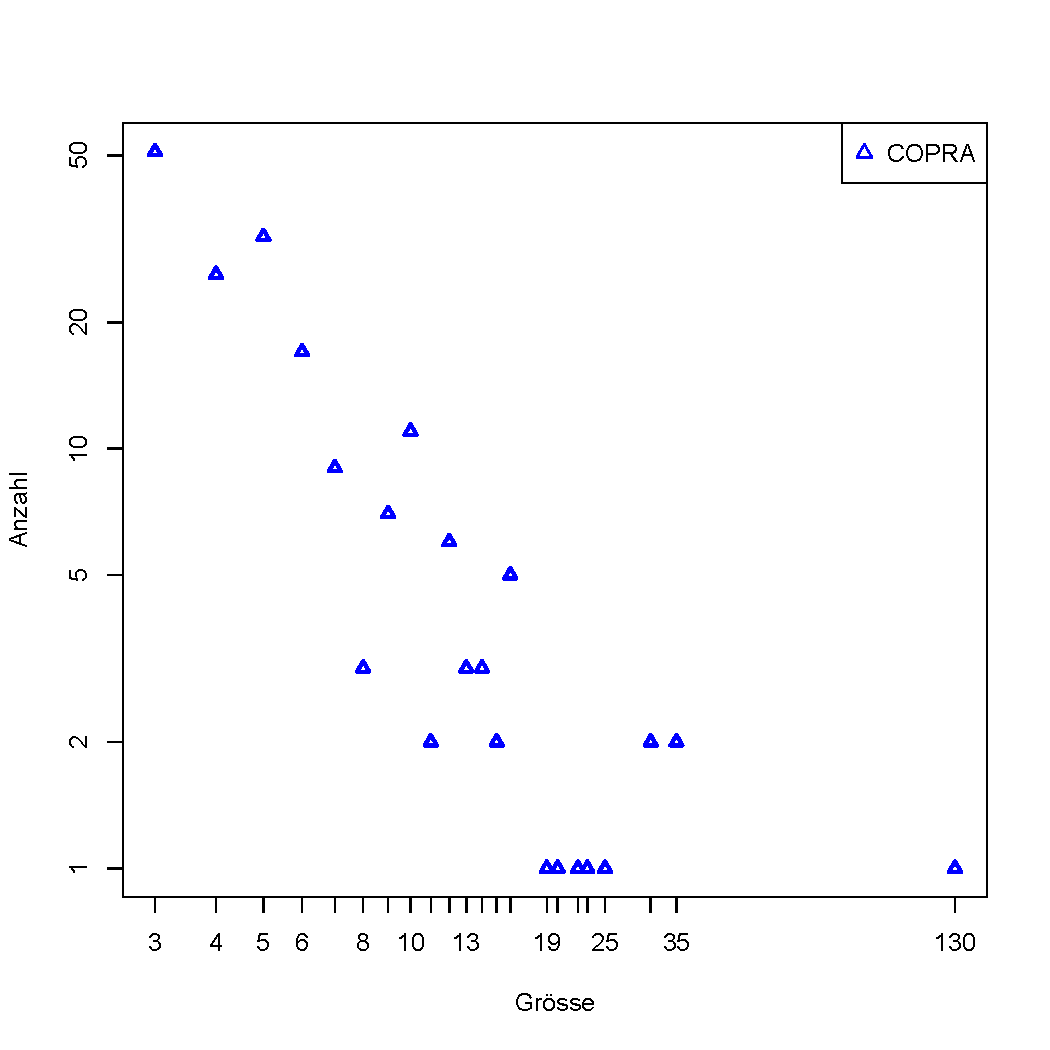
\includegraphics[scale=0.45]{images/sld-sure-ass_copra.pdf}}\\
  \subfloat[]{\label{fig:sld-sure-bl5} 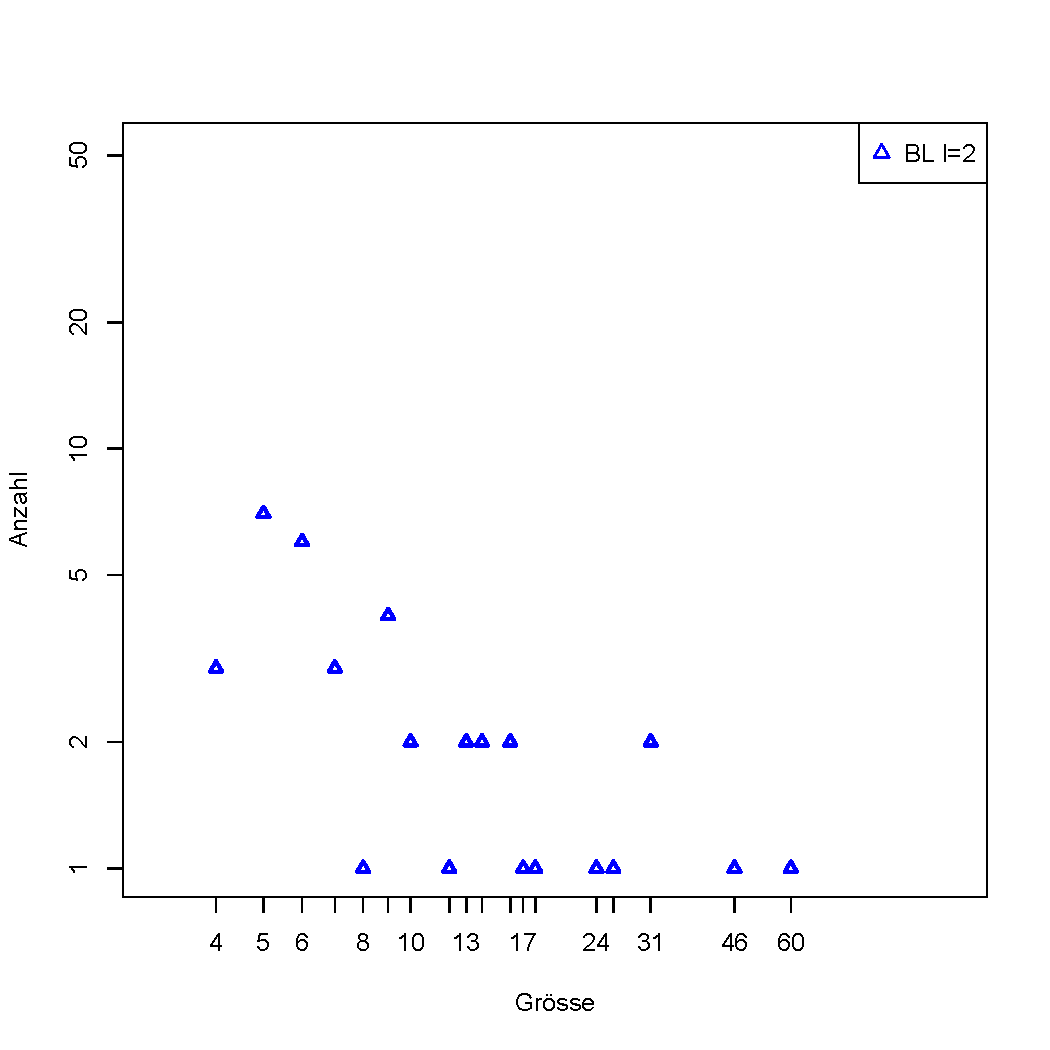
\includegraphics[scale=0.45]{images/sld-sure-ass_bl2.pdf}} 
  \subfloat[]{\label{fig:sld-sure-copra} 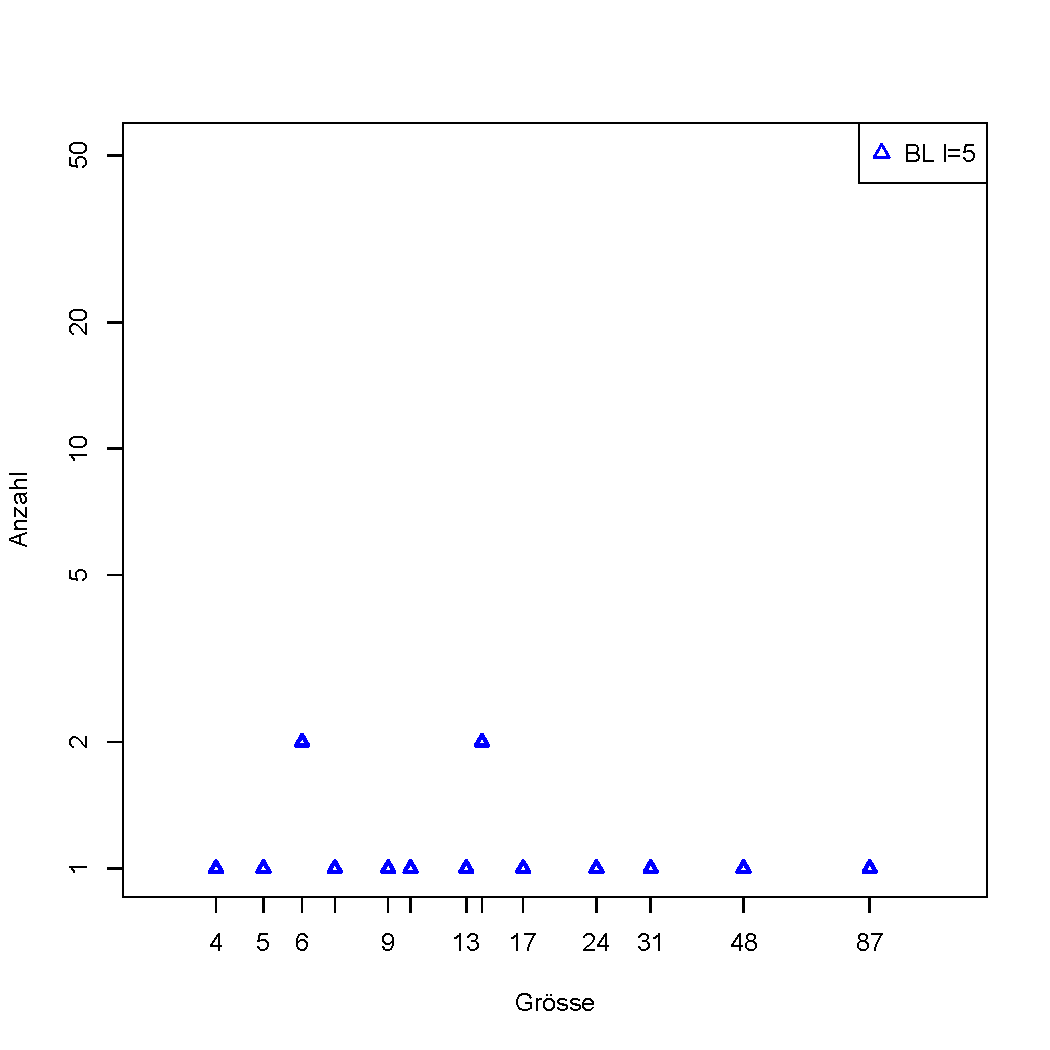
\includegraphics[scale=0.45]{images/sld-sure-ass_bl5.pdf}}
  \caption{Zuweisung von Domains zu SLDs abh\"angig von der Community-Gr\"osse}
  \label{fig:sld-suredist}
\end{figure}

\begin{figure}[t]
  \centering
  \subfloat[]{\label{fig:sld-maybe-copra1} 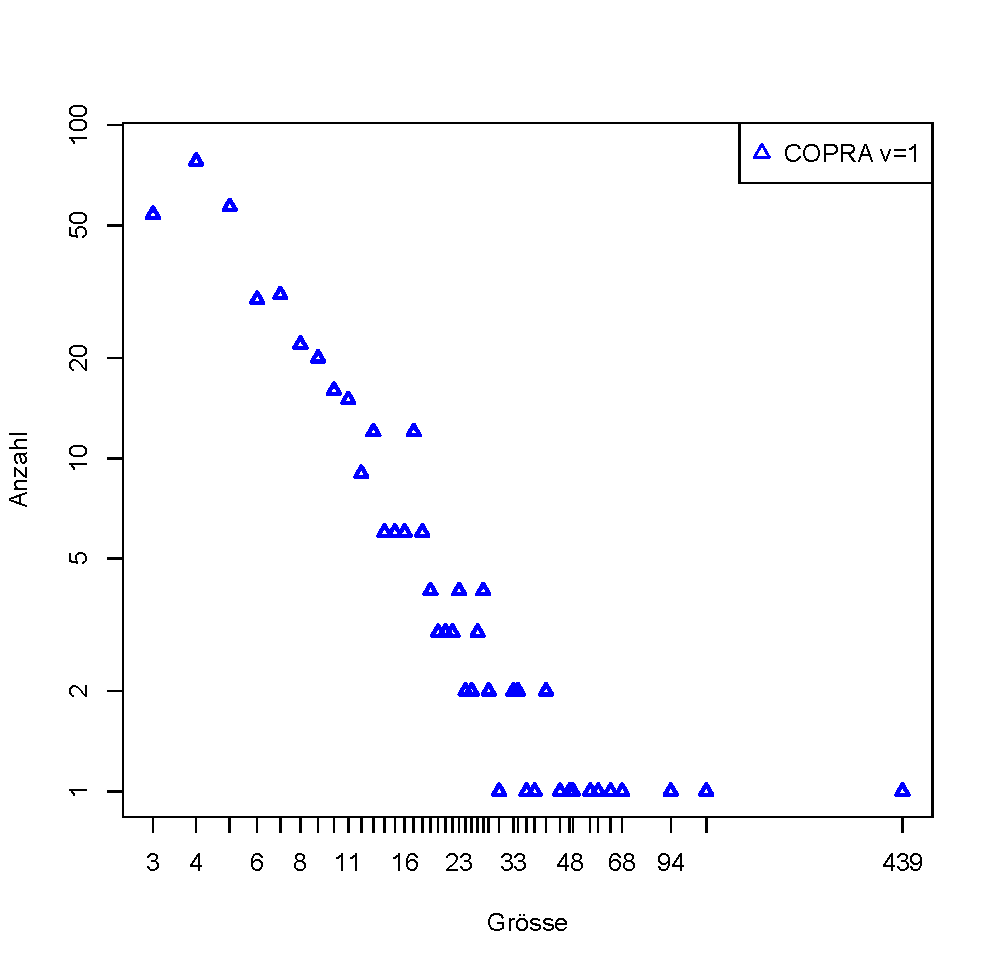
\includegraphics[scale=0.45]{images/sld-maybe-ass_copra1.pdf}}
  \subfloat[]{\label{fig:sld-maybe-bl2} 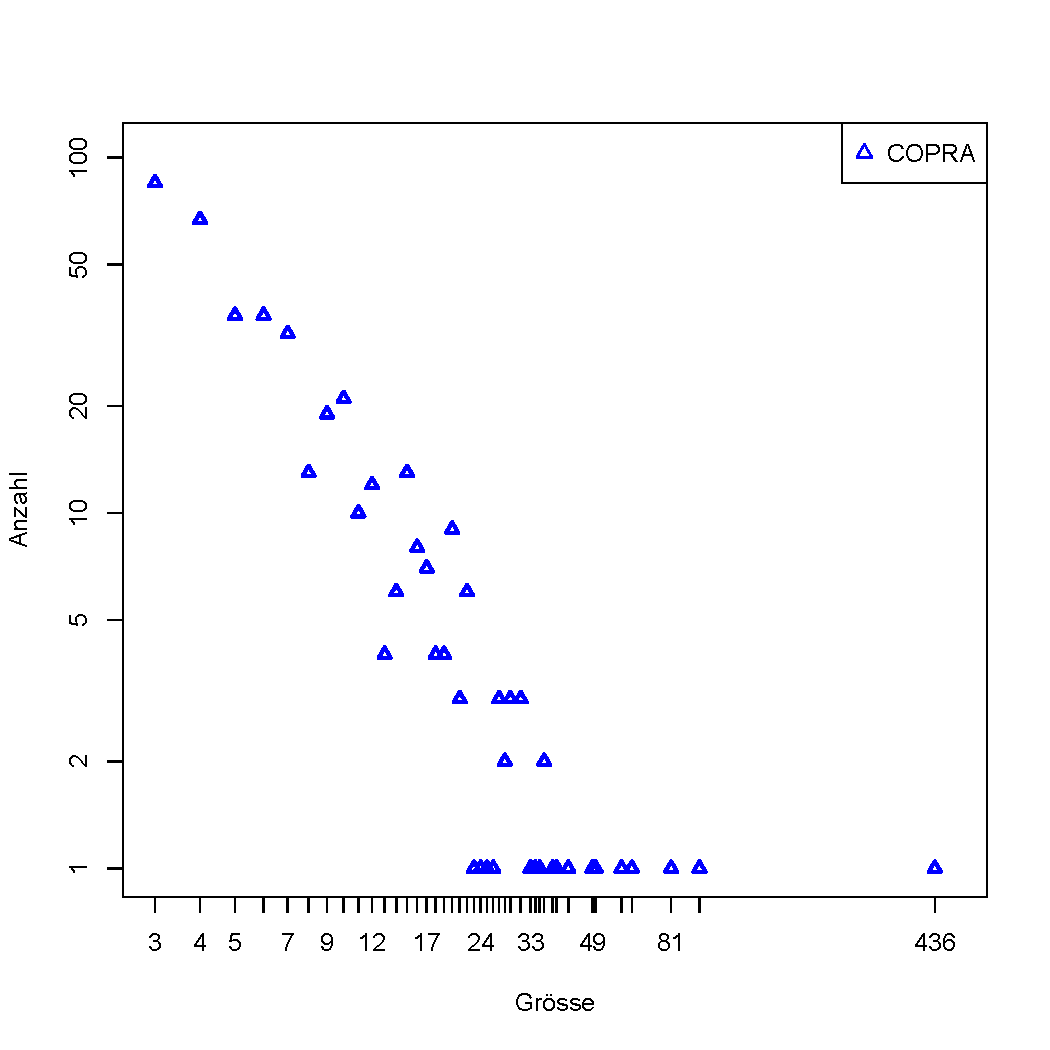
\includegraphics[scale=0.45]{images/sld-maybe-ass_copra.pdf}}\\
  \subfloat[]{\label{fig:sld-maybe-bl5} 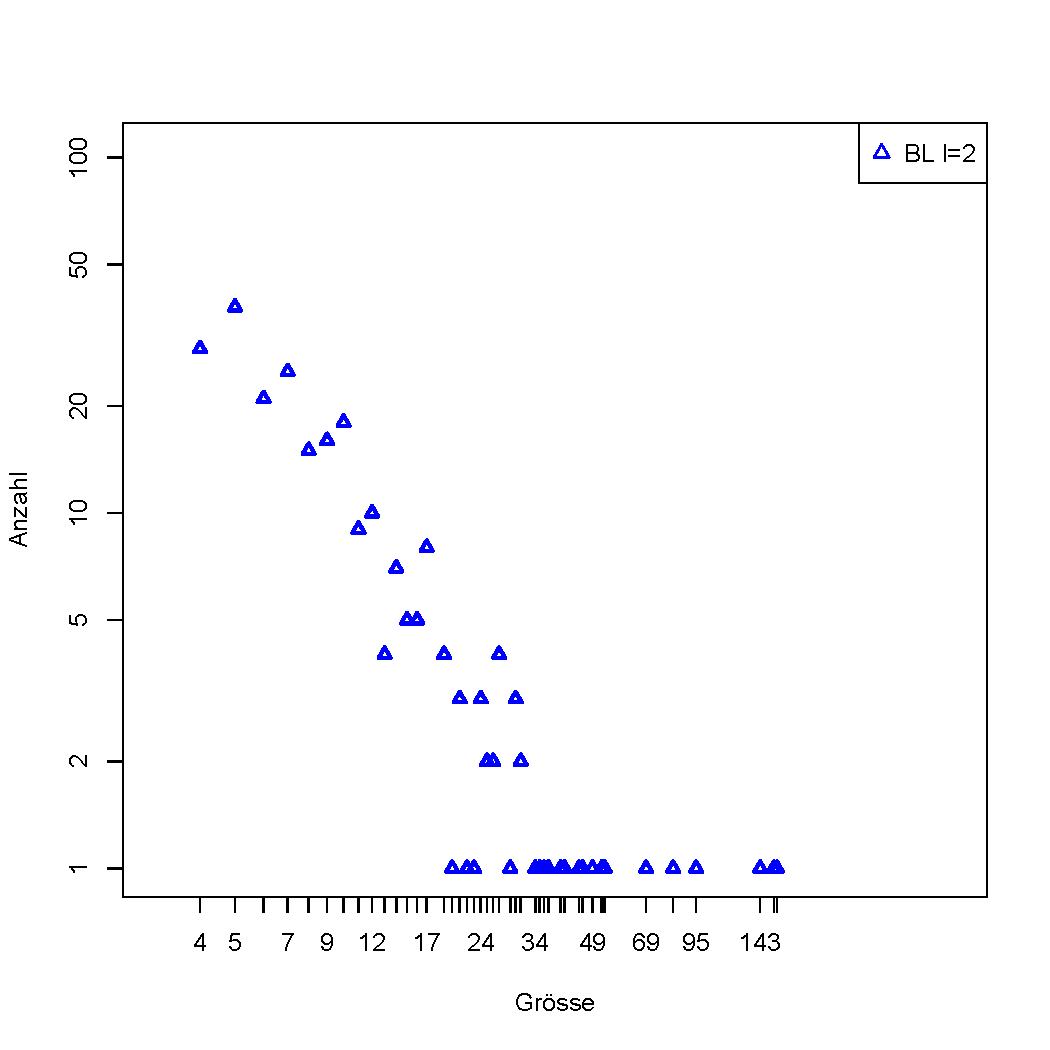
\includegraphics[scale=0.45]{images/sld-maybe-ass_bl2.pdf}} 
  \subfloat[]{\label{fig:sld-maybe-copra} 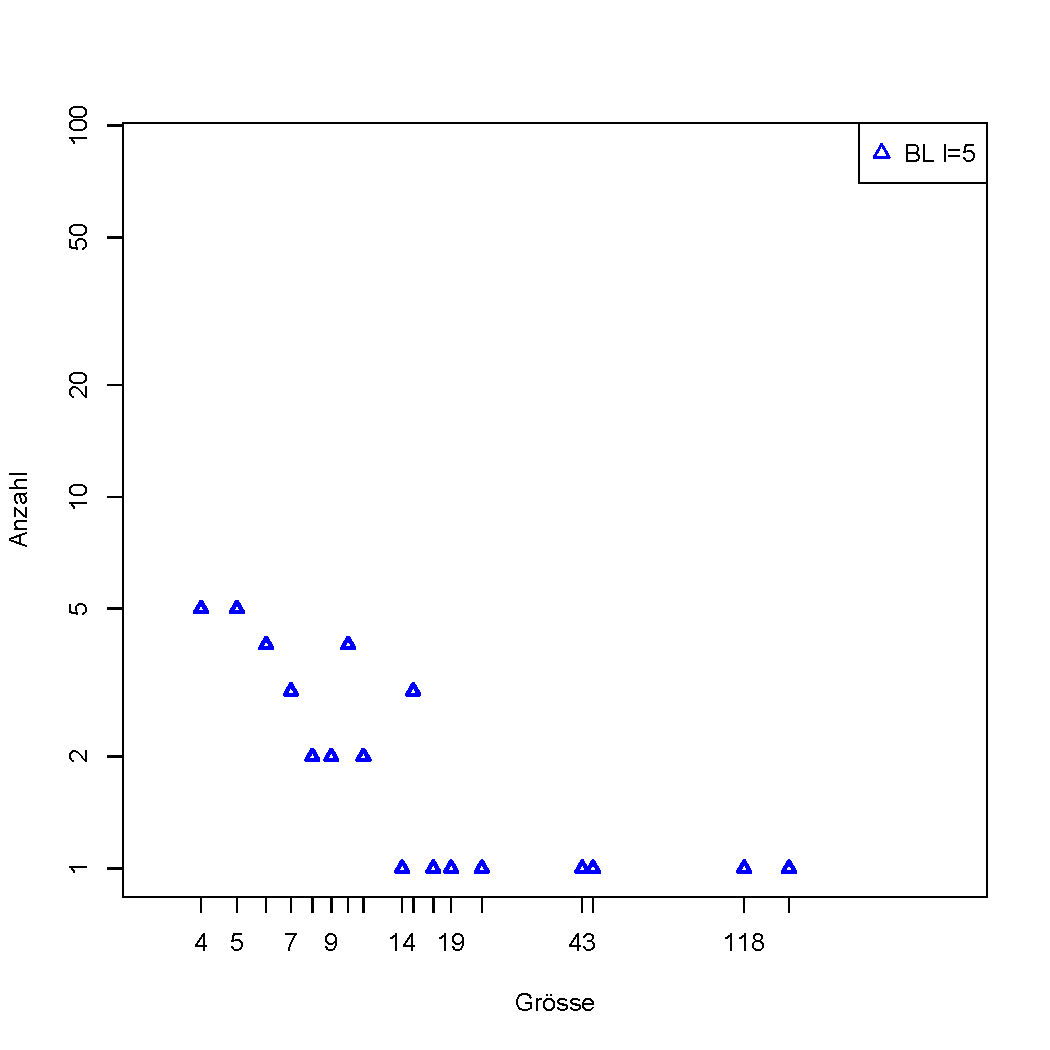
\includegraphics[scale=0.45]{images/sld-maybe-ass_bl5.pdf}}
  \caption{Verteilung der Gr\"osse der von einer SLD dominierten Communities}
  \label{fig:sld-maybedist}
\end{figure}

\begin{figure}[t]
  \centering
  \subfloat[]{\label{fig:time-corr-copra1} 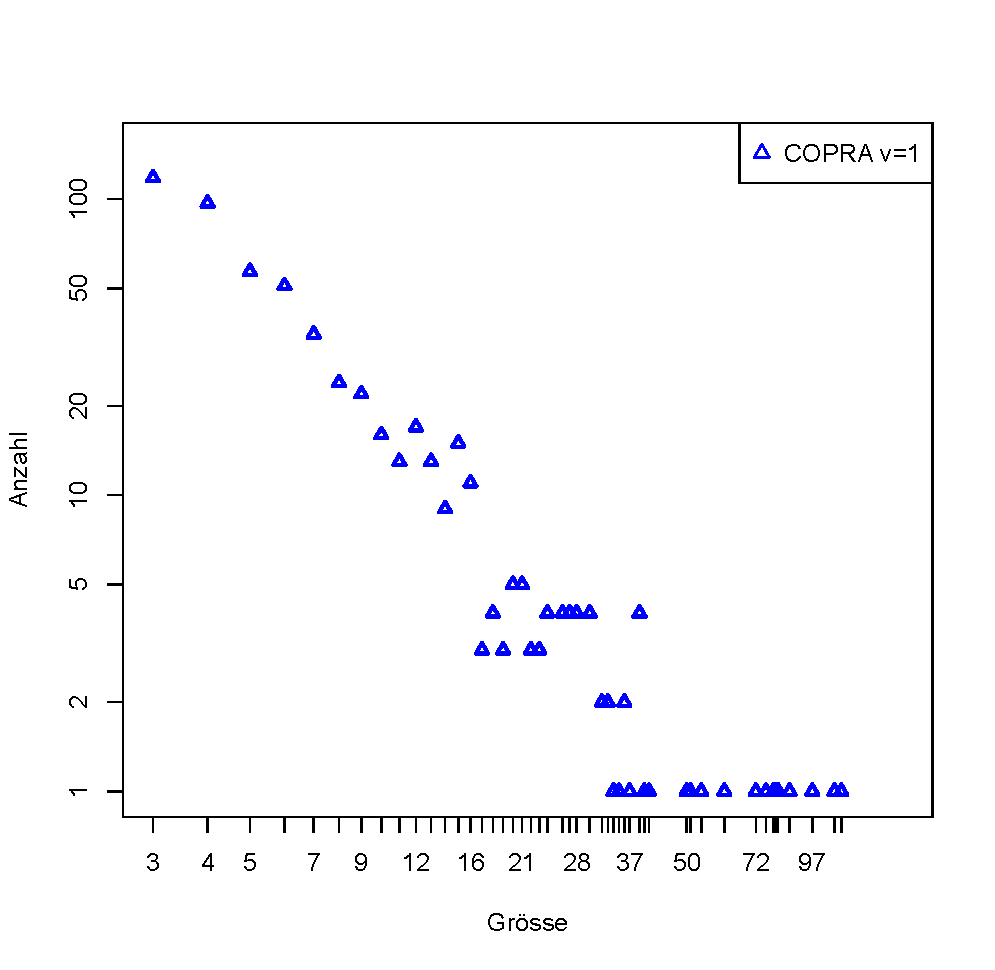
\includegraphics[scale=0.45]{images/time-corr_copra1.pdf}}
  \subfloat[]{\label{fig:time-corr-bl2} 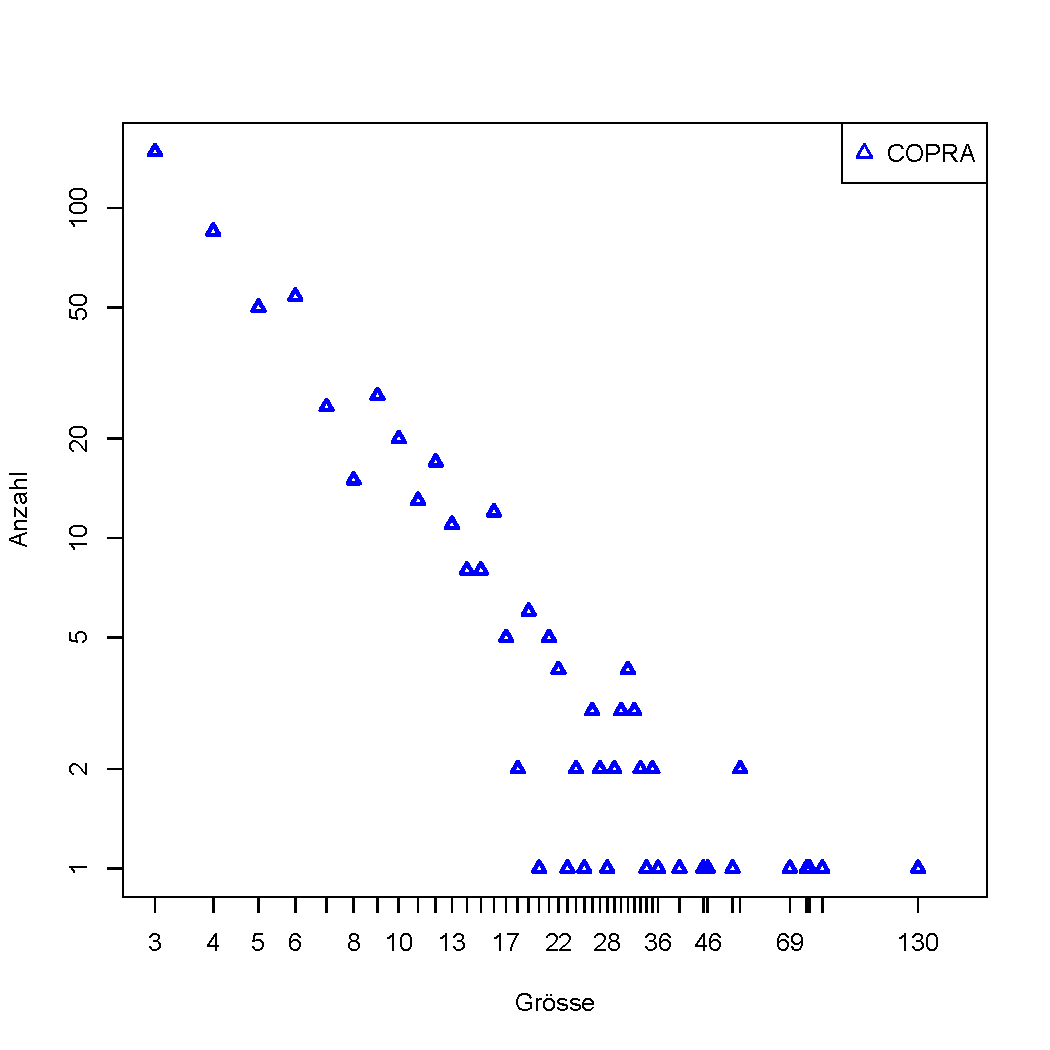
\includegraphics[scale=0.45]{images/time-corr_copra.pdf}}\\
  \subfloat[]{\label{fig:time-corr-bl5} 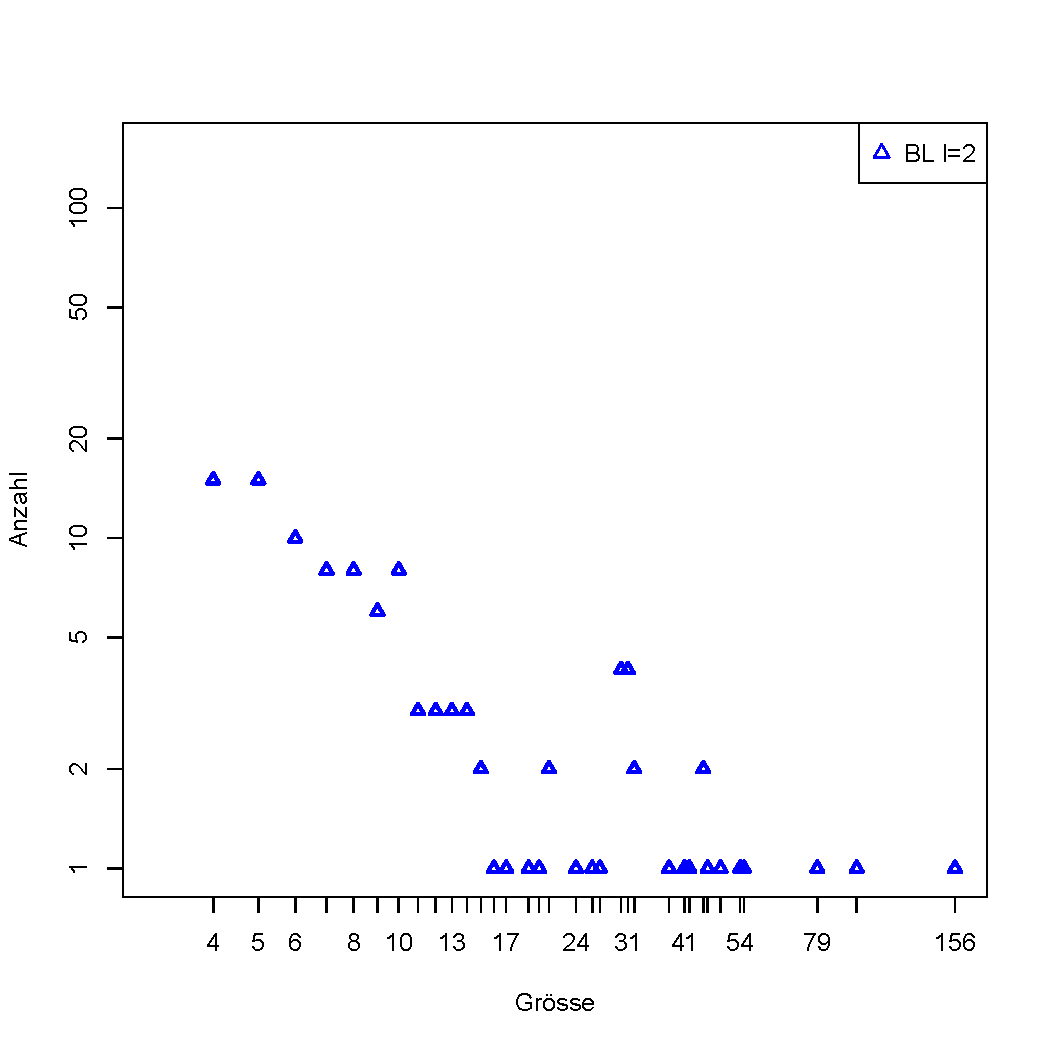
\includegraphics[scale=0.45]{images/time-corr_bl2.pdf}} 
  \subfloat[]{\label{fig:time-corr-copra} 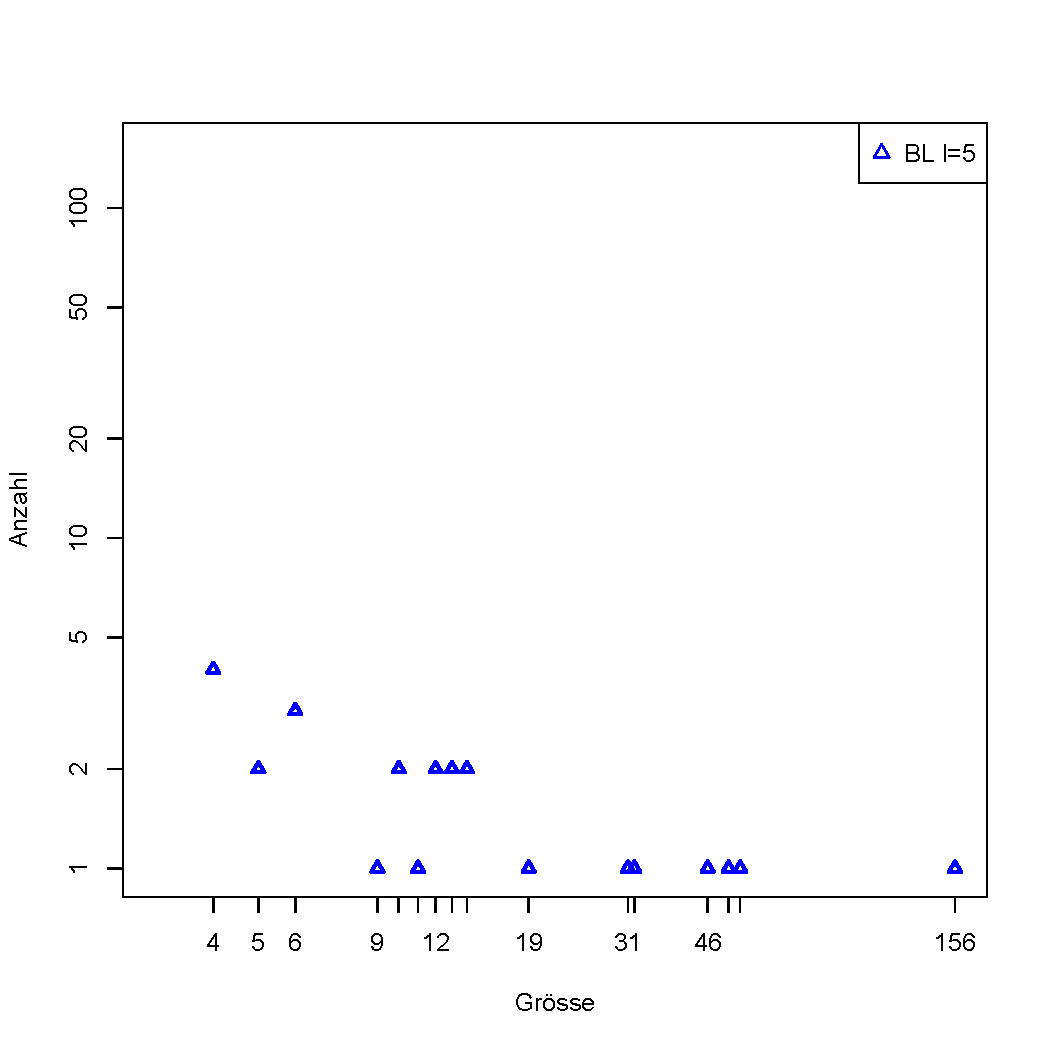
\includegraphics[scale=0.45]{images/time-corr_bl5.pdf}}
  \caption{Verteilung der Gr\"osse von Communities mit zeitlicher
    Korrelation der Signaturen}
  \label{fig:time-corrdist}
\end{figure}
Teilnehmer einer KSP, die schon gut vernetzt sind, werden ihre grosse
Community ja nicht einfach verlassen. Statt dessen wird die ``neue''
Community zur grossen hinzugef\"ugt oder so.

Zusammenfassung Allgemein: modulare Struktur, im Metagraphen keine
Sternstruktur sondern Vernetzung auf allen Gr\"ossenebenen. Bei 

(Kurzzusammenfassung: die Zuordnungszahlen sind niedrig. Tatsaechlich
zugeordnete Comm. (von nichttrivialer Groesse) sind dann aber auch
inhaltlich sinnvoll (KSPs mit fast-cliquenstruktur usw). Ausserdem:
optimale/bessere Zerlegung anhand von Modularity ist nicht automatisch
auch eine besser inhaltlich interpretierbare Zerlegung. Reduzierung
der Aufl\"osung kann zwar ``bessere'' Zerlegung ergeben, die aber
inhaltlich weniger aussagekr\"aftig ist. Ausserdem: kein signifikanter
Overlap. Und: unterschiedliche Algorithmen ``konvergieren'' nicht,
sondern liefern auch qualitativ unterschiedliche Ergebnisse (Blondel
<-> COPRA)

Diese Ergebnisse widerlegen nicht die Annahme, dass die
Vernetzung im Web of Trust im wesentlichen von Keysigning-Parties und
den sozialen Kontakten der Teilnehmer und damit unter anderem anhand
von Gruppenzugeh\"origkeit verl\"auft. Allerdings muss festgehalten
werden, dass die hier verwendeten Methoden nicht geeignet sind, um den
Entstehungsmechanismus entlang dieser Annahme befriedigend zu
erkl\"aren. 

Ein Grund daf\"ur ist sicherlich, dass die Struktur des Web of Trust
nur zu einem bestimmten, festen Zeitpunkt betrachtet wurde. Um die
Entstehungsdynamik zu verstehen, k\"onnte alternativ die Entwicklung
des Netzwerks tats\"achlich \"uber die Zeit nachvollzogen werden. Das
Keyserver-Netzwerk speichert nicht nur den momentanen Zustand des
Netzwerks, sondern implizit auch den Entstehungszeitpunkt jedes
Schl\"ussels und jeder Signatur. Die im Rahmen dieser Arbeit
entwickelte Software speichert diese Zeitstempel in einer Datenbank
und macht so die gesamte Entwicklungsgeschichte des Web of Trust
verf\"ugbar (siehe Abschnitt
\ref{ch:Grundlagen:sec:Design:subsec:eigene-software}). Anhand dieser
Daten k\"onnte nachvollzogen werden, wie und in welcher Form die
Communities tats\"achlich entstehen und sich entwickeln.

Mitgliedschaft in einer Gruppe (hier Firma, Open-Source-Projekt)
charakterisiert die sozialen Verbindungen einer Person nicht
vollst\"andig oder deutlich.

Das Problem im Ansatz ist, dass das WoT als Netz von building-blocks
(communities) gedacht wird, die entstehen und dann keine oder wenig
weitere Aktitiv\"at zeigen. Das Bild zeigt, dass das f\"ur einen
gewissen Teil (die, die teil einer ksp oder sld-s/m com sind) auch
zutrifft. allerdings gilt f\"ur einen sehr grossen Teil (21000 in
Monster-Community), offensichtlich, dass die Vernetzung so
vielf\"altig ist, dass solche primitive Mechanismen (KSPS + SGs) nicht
mehr sichtbar sind und in der Masse verschwinden.


%%% Local Variables: 
%%% mode: latex
%%% TeX-master: "diplarb"
%%% End: 

